\chapter{Establishing a Baseline Performance}

% \epigraph{\itshape Success is built sequentially. It's one thing at a ti me.}{---Gary W. Keller}

The objective of this thesis is to enhance the classification of underwater acoustic signals by refining preprocessing techniques and feature extraction methods. As with any scientific endeavour, it is essential to first establish a benchmark -- a reference point that serves as the foundation for measuring progress. This chapter lays out the baseline classifier architecture that will be used consistently throughout all subsequent experiments. By keeping the classifier architecture constant, we ensure that any performance improvements are solely attributed to changes in the preprocessing or feature extraction methods, rather than from adjustments in the classifier.

This chapter is organised as follows. We begin by introducing the dataset, detailing the process of segmenting it into folds to enable cross-validation during training. We also examine the class distribution across the dataset and within each fold, identifying any imbalances that may influence model performance.

Next, we describe the chosen classifier architecture -- a hybrid \acrshort{cnnlstm} model that combines the spatial feature extraction capabilities of convolutional layers with the temporal pattern recognition strengths of \acrshort{lstm} layers. This model will serve as the foundation for all further experiments in this thesis. We discuss the feature inputs for the model, specifically the power spectrograms derived from each audio sample, and outline the process of extracting these using MATLAB, including key parameters such as the \acrshort{fft}, window size, overlap percentage, and frequency resolution. 

Lastly, we cover the approach to hyperparameter tuning to maximise the model's baseline performance. We conclude with a discussion of the coding frameworks and libraries used, as well as the hardware setup, including the GPU utilised for training. This ensures a comprehensive understanding of the baseline model's development, configuration, and evaluation.

%%%%%%%%%%%%%%%%%%%%%%%%%%%%%%%%%%%%%%%
\section{The dataset: DeepShip}

The dataset selected for this study is the DeepShip dataset \cite{irfan_deepship_2021}. There are two key reasons behind this choice. Firstly, DeepShip has become the authoritative benchmark dataset for \acrshort{uatr}, with many recent scientific studies reporting their performance metrics on this dataset. Given its extensive use, the dataset provides a solid foundation for evaluating new techniques, allowing direct comparison with a vast body of prior work. Additionally, past research students at Thales have also worked with DeepShip, publishing their findings, which provides continuity for our work and the opportunity to build upon their results.

Secondly, while the newly released OceanShip dataset (see Section \ref{subsubsec:oceanship}) offers more recordings than DeepShip -- over twice the length in minutes -- it is currently inaccessible due to issues with the international accessibility of the cloud storage provider chosen by its authors. More importantly, the class labels within OceanShip have not been externally validated, raising concerns over the quality and reliability of its data. In contrast, DeepShip has undergone independent verification by sonar processors at Thales, ensuring its labels are accurate and reliable for research purposes.

\subsection{Dataset overview}

As outlined in Section \ref{subsubsec:deepship}, the DeepShip dataset consists of 613 recordings from 265 ships, categorised into four vessel classes (see Table \ref{tab:deepship-summary} for more information). However, some of the recordings in the original dataset lack metadata, leading us to work with a refined subset of DeepShip for this thesis. This subset includes 582 of the 613 recordings, representing 249 of the 265 vessels. Consequently, the dataset length is slightly reduced to 2684 minutes, compared to the original 2824 minutes. Table \ref{tab:deepship-subset} compares the number of ships, recordings, and total recording time for each vessel class in our subset (values outside parentheses) with the original dataset (values inside parentheses). Hereafter, this subset will be referred to simply as DeepShip.

\begin{table}[h]
\centering
\begin{tabular}{llll}
\toprule
\textbf{Vessel class} & \textbf{Ships} & \textbf{Recordings} & \textbf{Total recording time (min)} \\ \midrule
Cargo & 62 (69) & 106 (110) & 628 (640) \\
Passengership & 43 (46) & 180 (193) & 715 (742) \\
Tanker & 128 (133) & 234 (240) & 735 (765) \\
Tug & 16 (17) & 62 (70) & 606 (677) \\
\textbf{Total} & \textbf{249 (265)} & \textbf{582 (613)} & \textbf{2684 (2824)} \\ \bottomrule
\end{tabular}
\caption{Comparison of the DeepShip subset used in this thesis (values outside parentheses) with the complete DeepShip dataset (values in parentheses).}
\label{tab:deepship-subset}
\end{table}

Like many real-world datasets, DeepShip exhibits a minor class imbalance, with some ship classes being more heavily represented than others. A class distribution analysis was conducted to visualise this imbalance. Figure \ref{fig:deepship-subset-recording-length} illustrates the variation in the duration of recordings for a vessel. As shown, there is at least one outlier vessel in each class that is significantly over-represented. For example, the median recording duration of all cargo vessels is 5.9 minutes, yet the cargo vessel \texttt{PRINCESS\_SUPERIOR} has over 151 minutes of sonar signal data. Also, the number of ships and number of recordings in each class is quite unbalanced (Figure \ref{fig:deepship-subset-number-vessels}), however the overall total recording time of each class is fairly balanced (Table \ref{tab:deepship-subset}).

\begin{figure}[p]
    \centering
    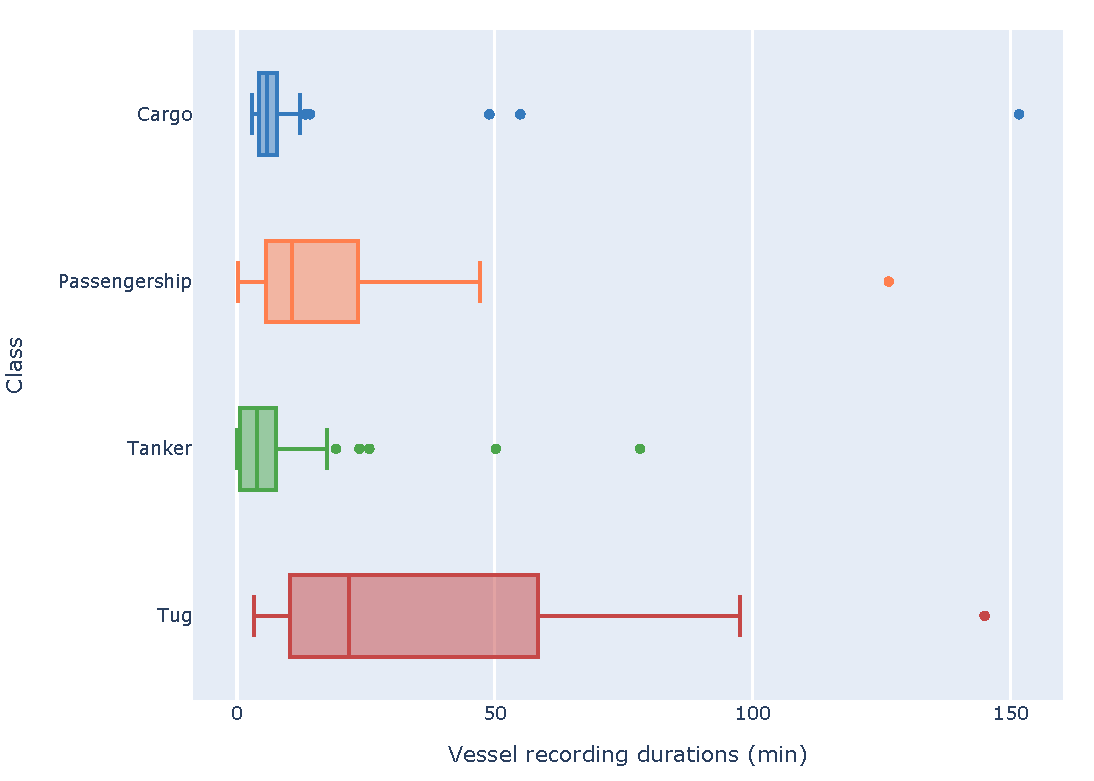
\includegraphics[width=0.95\textwidth]{img/ch3/deepship_duration_spread.pdf}
    \caption{The distribution of vessel recording durations in the DeepShip subset, split by class.}
    \label{fig:deepship-subset-recording-length}
\end{figure}

\begin{figure}[p]
    \centering
    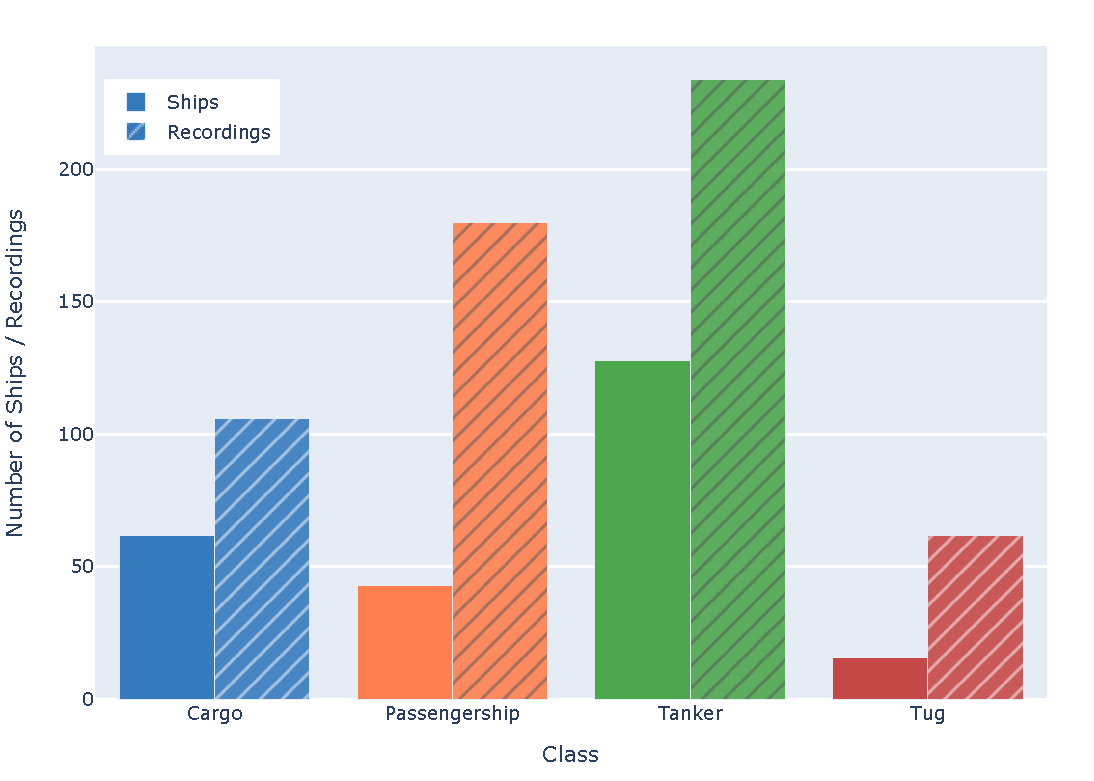
\includegraphics[width=0.95\textwidth]{img/ch3/deepship_class_analysis.pdf}
    \caption{The number of vessels and number of recordings in each class of the DeepShip subset, split by class.}
    \label{fig:deepship-subset-number-vessels}
\end{figure}

\subsection{Recording segmentation}\label{subsec:segmentation}

A widely used approach in audio applications for machine learning is to split each audio recording into smaller segments to boost the number of training samples, improve granularity in feature extraction, and allow more robust classification models to be trained. Segmenting the data into smaller clips enables better generalisation by providing the model with more diverse examples and variations across the data. Additionally, smaller, more homogeneous segments can allow the model to focus on the most relevant features while ignoring background noise components, thereby improving classification performance \cite{xu_self-supervised_2023}. Some examples of \acrshort{uatr} literature which employ segmentation on the DeepShip dataset include: Li et al. \cite{li_underwater_2022}, who segmented the DeepShip dataset into 5-second clips to yield 11,174 samples, using a 70-20-10 split for training, verification, and test datasets respectively; Chen et al. \cite{chen_hierarchical_2024}, who segmented DeepShip into 5-second segments and then divided each class into five equal folds at random; and Sun and Leo \cite{sun_underwater_2023}, who used a 3-second segmentation strategy for DeepShip, acknowledging the importance of segmenting audio to increase the number of samples and make the dataset more computationally feasible for machine learning models. 

The choice of 3-second segments, specifically, is also grounded in previous studies, which have demonstrated that this interval strikes an optimal balance between maintaining sufficient audio context for accurate classification and also managing the model's computational complexity. Longer segments may provide more stability and context, however they also increase computational demands and the risk of overfitting by capturing more irrelevant or noisy information \cite{chen_ship-radiated_2024, li_underwater_2022}. Conversely, shorter segments may lack sufficient context, with burst noise or transient phenomena in the signal having a more pronounced negative impact on classification accuracy \cite{shen_auditory_2018, tang_deep_2024}. Thus, the 3-second segment length aims to achieve an effective balance between data complexity and computational efficiency. This segment length is consistent with other state-of-the-art studies that similarly found 3-second segments optimal for underwater acoustic target recognition tasks \cite{xu_self-supervised_2024, tang_deep_2024}. Notably, the original authors of the DeepShip dataset also chose to divide each recording into 3-second segments, further validating this selection \cite{irfan_deepship_2021}.

In total, DeepShip, with a total recording time of 2684 minutes (161,040 seconds), was segmented into 53,680 3-second segments. After removing segments containing only background noise or silence -- to ensure that the inputs were actually representative of ship noise patterns -- there were a total of 53,503 valid segments remaining.

\subsection{Distribution of segments into folds}

In auditory applications of machine learning, it is common practice to divide input audio clips into $k$ folds for cross-validation \cite{chi_classifying_2022, basili_classification_2004, zeng_spectrogram_2019, chen_ship-radiated_2024, chen_hierarchical_2024}. The most common approach is \textit{leave-$p$-out cross-validation}, where $p$ folds are used for training and the remaining $k-p$ folds for testing. This process is repeated until each fold has been used for both training and testing. In cases where the dataset allows, \textit{stratified $k$-fold cross-validation} is preferred, as it ensures that each fold contains an equal number of samples from each class. However, this ideal design is not always feasible due to the original dataset's class distribution.

Hence, following best practice, after segmentation the dataset was divided into 10 folds with an effort to maintain an approximately equal number of 3-second segments from all four ship classes in each fold. A Python script was used to automate this process, generating a CSV file that specifies the assignment of each 3-second segment to a fold.

Two key considerations guided the design of the 10-fold split for DeepShip. First, to prevent the model from learning recording-specific characteristics, such as background noise or vessel-specific nuances, all clips derived from a given recording were placed in the same fold \cite{chi_classifying_2022}. Second, given that \acrshort{uatr} datasets often contain multiple recordings from the same vessels, we aimed to distribute an approximately equal number of samples from each vessel across the folds. This not only helps balance the class distribution within each fold but also ensures that each vessel is consistently represented across the folds, improving the robustness of the model evaluation.

It should be noted, however, that the split is not perfectly uniform; some variability exists in the number of segments per fold. For instance, the Tug class exhibits the largest variation, with Fold 1 containing only 360 segments, while Fold 3 contains 3006. The complete distribution of samples across the 10 folds is shown in Figure \ref{fig:10-fold-overview}. This variability arises from the constraints mentioned above: entire recordings, rather than individual segments, were assigned to each fold to avoid splitting a recording across multiple folds. Furthermore, efforts to distribute an equal number of samples from each vessel across the folds were limited by the inherent imbalance in recording durations within the DeepShip dataset (Figure \ref{fig:deepship-subset-recording-length}). Despite the resulting variability, this method still enhances the dataset's integrity by ensuring that no recording is split across multiple folds, ultimately improving the consistency and robustness of the dataset for cross-validation.

\begin{figure}[htbp]
    \centering
    % Subfigure 1: Fold counts by class
    \begin{subfigure}[t]{\textwidth}
        \centering
        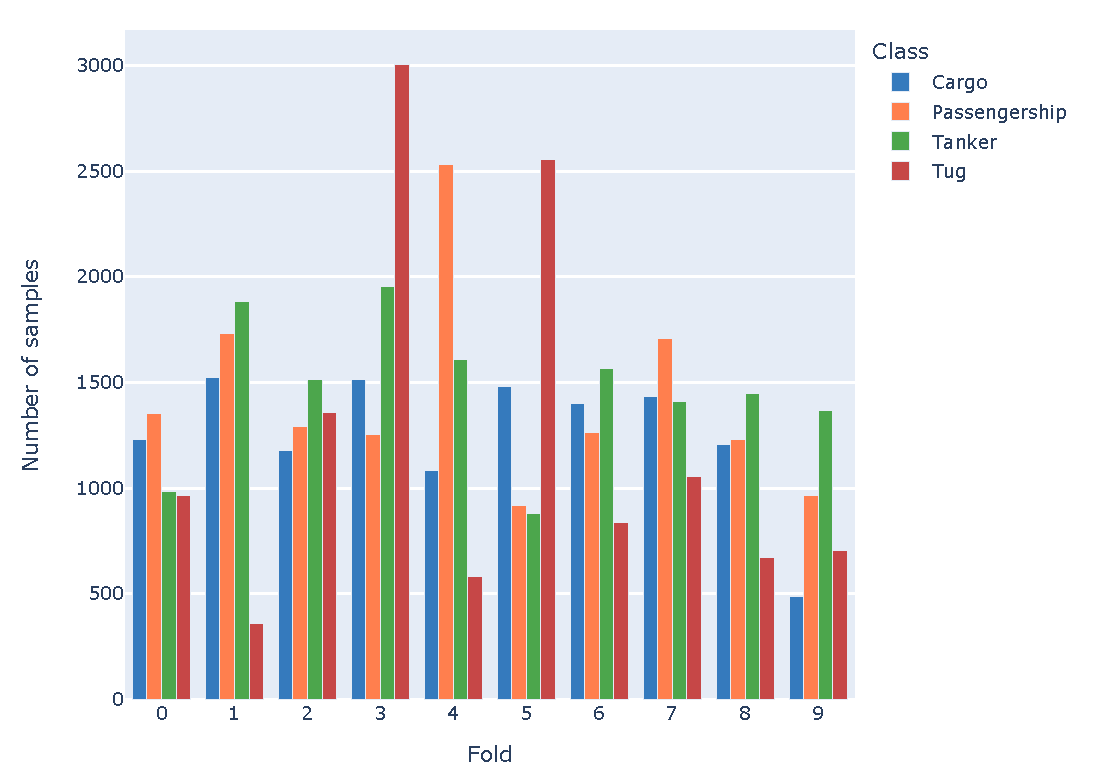
\includegraphics[width=0.95\textwidth]{img/ch3/10_folds_counts.pdf}
        \caption{Count of samples in each fold by class}
        \label{fig:10-fold-counts}
    \end{subfigure}

    \vspace{1cm}
    
    % Subfigure 2: Sample counts by fold 
    \begin{subfigure}[t]{\textwidth}
        \centering
        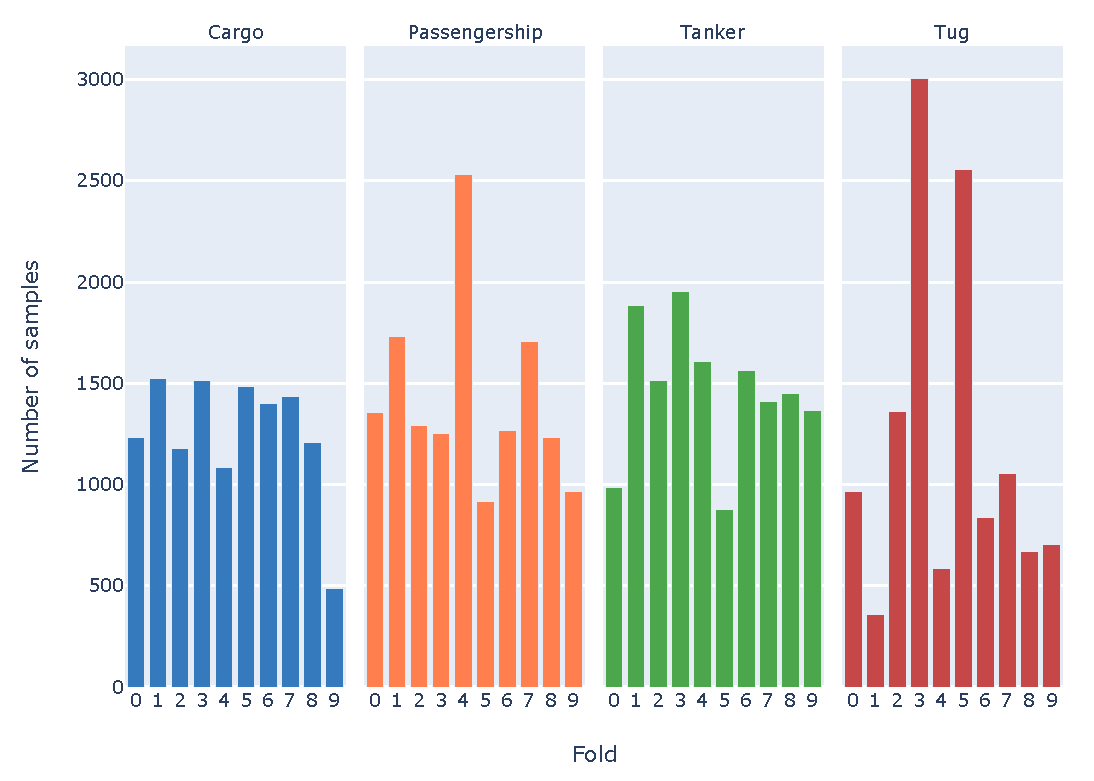
\includegraphics[width=0.95\textwidth]{img/ch3/10_fold_counts_facet.pdf}
        \caption{Count of samples in each class by fold}
        \label{fig:10-fold-counts-facet}
    \end{subfigure}
    \vfill
\end{figure}
\begin{figure}
    \ContinuedFloat
    % Subfigure 3: Spread of samples per class
    \begin{subfigure}[t]{\textwidth}
        \centering
        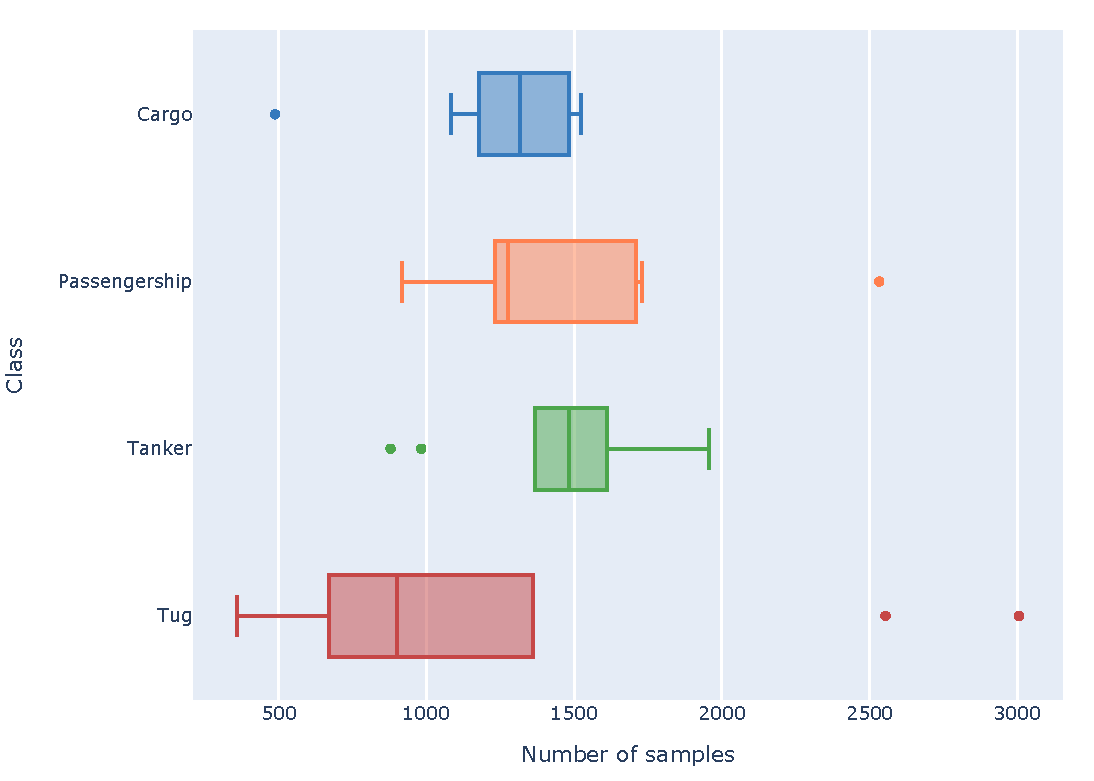
\includegraphics[width=0.95\textwidth]{img/ch3/10_fold_spread.pdf}
        \caption{Spread of samples in each fold by class}
        \label{fig:10-fold-spread}
    \end{subfigure}
    \caption{Distribution of samples across 10-fold split.}
    \label{fig:10-fold-overview}
\end{figure}

\subsection{Other standardised approaches}

Given the significant variation in segmentation and splitting methodologies highlighted by Niu et al. \cite{niu_advances_2023}, there has been a recent trend towards adopting standardised train-test splits to enable more direct comparisons between classification techniques. In 2023, Zhu et al. proposed a specific division of the DeepShip dataset into 3-second segments for a consistent training and testing split \cite{zhu_underwater_2023}. This standardised split was published online \cite{zhupengsen_zhupengsenmethod-for-splitting--deepship-dataset_2024}, and several subsequent studies have since adopted this methodology to ensure comparability across research \cite{xu_self-supervised_2023, xu_self-supervised_2024, zhu_sfc-sup_2023, lin_underwater_2024}.

Zhu et al. also introduced a standardised background noise class to complement the DeepShip dataset. Unlike other datasets such as QiandaoEar22 (see Section \ref{subsubsec:qiandaoear22}), DeepShip lacks a dedicated background noise class due to the high level of shipping activity in the recording area, which means all recordings contain some degree of ship noise \cite{irfan_deepship_2021}. Although the original authors of DeepShip used over seven hours of external background noise recordings in their classifier, they did not disclose or publish these files. To address this, Zhu et al. provided a set of background noise files for future studies.

However, the inclusion of external background noise remains a point of debate. Some researchers, such as Tian et al., have incorporated background noise to improve classification performance \cite{tian_joint_2023}. However, others argue that this approach may not accurately reflect the specific acoustic environment of the DeepShip recordings.

For this study, we adhered to our own splitting methodology, consistent with the practices of Thales researchers, to maintain continuity across our internal projects. Furthermore, we opted not to augment the dataset with random noise samples, as we do not consider this step necessary or appropriate for accurately reflecting the operational environment represented in DeepShip.

%%%%%%%%%%%%%%%%%%%%%%%%%%%%%%%%%%%%%%%
\section{Input features}\label{sec:inputs}

The input feature chosen for our benchmark model was the power spectrogram, a transformed version of the conventional spectrogram designed to enhance interpretability and align with human auditory perception. Power spectrograms apply a logarithmic transformation to the conventional spectrogram, calculated as $10 \cdot \log_{10}(P + \epsilon)$, where $P$ is the power or magnitude of the signal and $\epsilon$ is a small constant to avoid zero values. This logarithmic scaling brings the power spectrogram more in line with human auditory perception and also emphasises subtler sound components, making it both more visually interpretable and informative for analysis. The decision to use power spectrograms is well-supported by existing literature in underwater acoustics. For instance, previous studies, such as Cao et al. \cite{cao_underwater_2019}, have demonstrated the use of power spectrograms for extracting unique frequency features associated with vessel machinery, like shaft frequencies. 

\subsection{Processing pipeline}

\subsubsection{Downsampling}

Each audio recording was downsampled from the original sampling rate of 32 kHz to 5 kHz. This choice was guided by studies such as Arveson and Vendittis \cite{arveson_radiated_2000}, Malinowski et al. \cite{malinowski_underwater_2001}, Pricop et al. \cite{pricop_underwater_2010}, and McKenna et al. \cite{mckenna_underwater_2012}, which suggest that the majority of discriminative acoustic information for modern commercial vessels lies within the 0-2 kHz frequency range. Hence, in-line with the Nyquist-Shannon sampling theorem, 5 kHz was chosen to maintain the most important frequency features whilst also reducing computational complexity. 

\subsubsection{Audio normalisation}

Each audio clip then underwent 0-1 normalisation to standardise amplitude levels across samples. This step aimed to mitigate the effects of loudness variations, allowing the machine learning model to focus on frequency-based characteristics rather than amplitude fluctuations.

\subsubsection{Spectrogram generation}

The spectrograms were computed using MATLAB's \texttt{spectrogram} function, with parameters fine-tuned over several iterations to achieve an optimal balance between time and frequency resolution. Table \ref{tab:powerspectrogram-parameters} lists the final parameters used for spectrogram generation.

\begin{table}[htbp]
    \centering
    \begin{tabular}{ll} \toprule 
    \textbf{Parameter} & \textbf{Value} \\ \midrule 
    Sampling frequency (\texttt{fs}) & 5 kHz \\ 
    Window length (\texttt{window}) & 40 ms = 200 segments, rounded to 256 segments \\ 
    Overlap (\texttt{noverlap}) & 75\% of window length \\ 
    FFT length (\texttt{nfft}) & 1024 points \\ 
    Output dimensions & $195 \times 231$ (frequency bins $\times$ time bins) \\ \bottomrule
    % Low-frequency cutoff (\texttt{startHz}) & 50 Hz \\
    % High-frequency cutoff (\texttt{stopHz}) & 1000 Hz \\
    % Spectrogram normalisation (\texttt{normaliseSpec}) & Disabled for baseline \\
    % Spectrogram resizing (\texttt{resize}) & 192x192 pixels \\ \bottomrule 
    \end{tabular}
    \caption{Final STFT parameters for power spectrogram computation.}
    \label{tab:powerspectrogram-parameters}
\end{table}

The window length of 40 milliseconds was selected to achieve a balance between frequency resolution (for capturing tonal components) and temporal resolution (for capturing transients). A 75\% overlap was applied between consecutive windows to minimise information loss, and the \acrshort{fft} length was set to 1024 points, providing sufficient spectral detail.

The output of the \texttt{spectrogram} function is $S$, the short-time Fourier transform of the input signal returned as a matrix. This output was subsequently converted into decibel scale using the transform $P = 10 \cdot \log_{10}(|S|^2 + 10^{-8})$.

\subsubsection{Amplitude cutoff}

To suppress low-intensity regions dominated by background noise, the spectrogram amplitudes were thresholded at a minimum of $-30$ dB. This threshold was chosen based on the analysis of amplitude distributions across all vessel classes. Figure~\ref{fig:ampl-cutoff-histogram} illustrates the average amplitude histograms for the four vessel classes, highlighting that the majority of amplitude values are concentrated between $-30$ dB and 20 dB. Cargo and Tanker classes exhibit the widest amplitude ranges, extending from approximately $-40$ dB to 30 dB, while Passengership and Tug classes display narrower ranges with fewer extreme values. Most importantly, amplitude values below $-30$ dB are uncommon, justifying the cutoff.

The main benefit of applying this threshold is that it removes the influence of an extremely small number of low-amplitude values ($<-30$ dB) on the color scaling of the spectrograms. This ensures a more uniform color mapping. Figure~\ref{fig:ampl-cutoff-spectrogram} compares spectrograms from the same recording with the same \acrshort{stft} parameters before and after applying the low amplitude cutoff. In the unprocessed spectrogram, the presence of low-intensity noise has a ``blurring'' effect on the figure, while the spectrogram with the cutoff highlights narrowband events with much greater sharpness and clarity.

\begin{figure}[htbp]
    \centering
    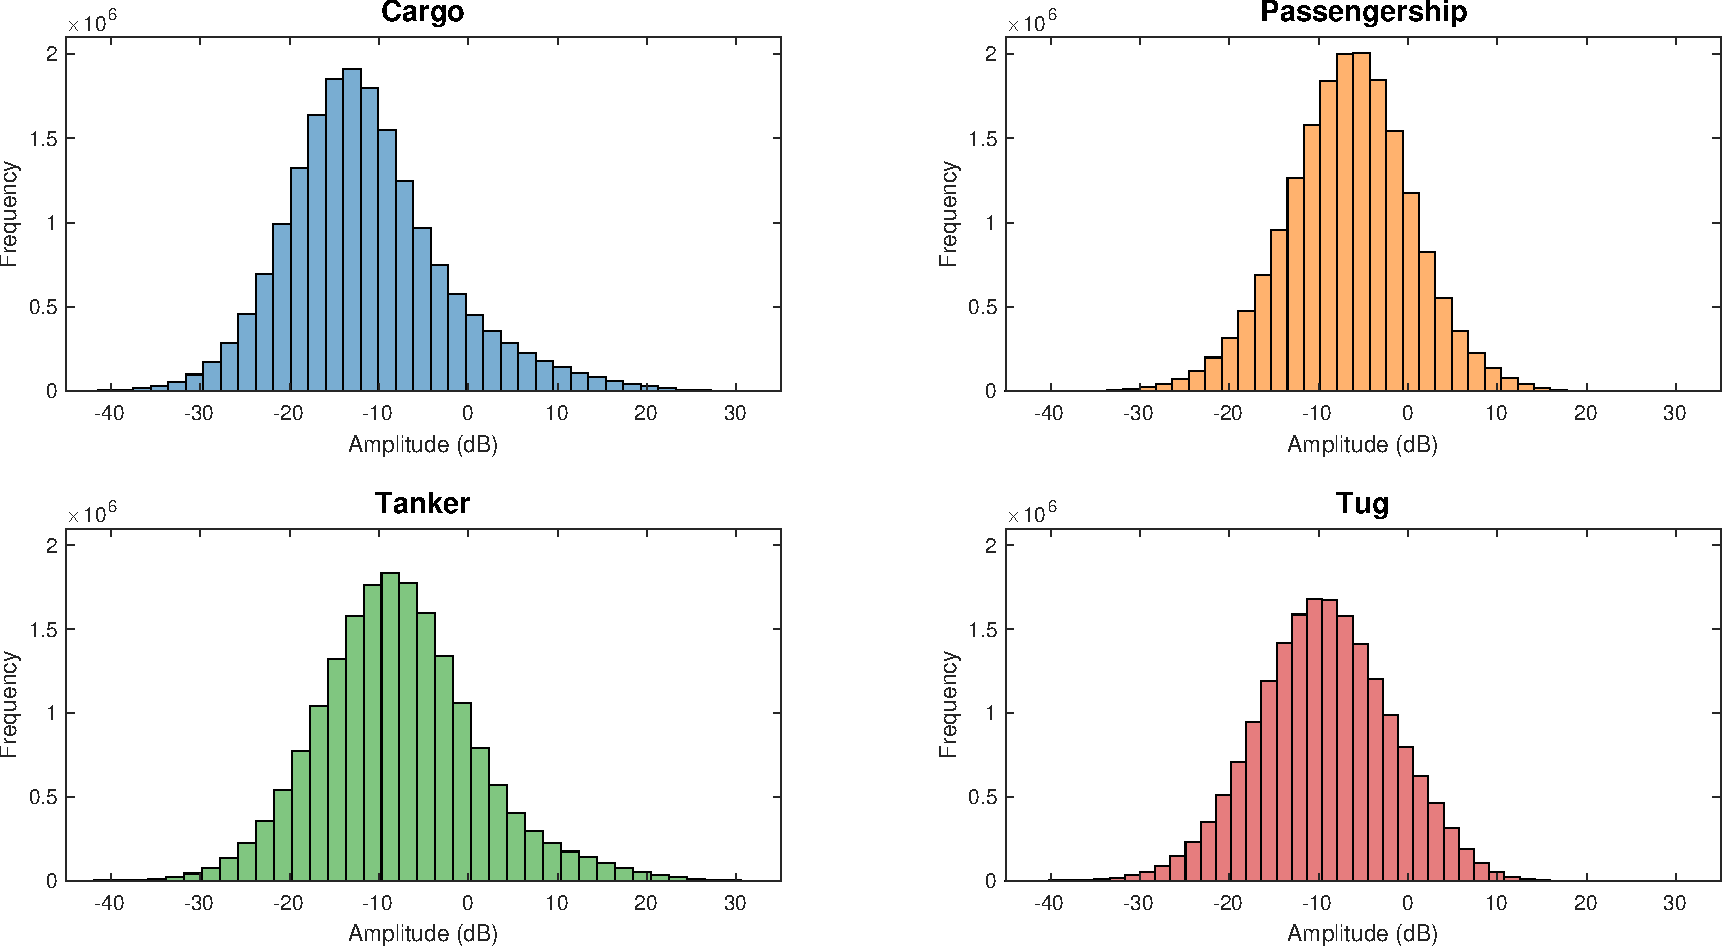
\includegraphics[width=\textwidth]{img/ch3/ampl_cutoff/averageHistogram.pdf}
    \caption{Average amplitude histograms for each vessel class.}
    \label{fig:ampl-cutoff-histogram}
\end{figure}

\begin{figure}[htbp]
    \centering
    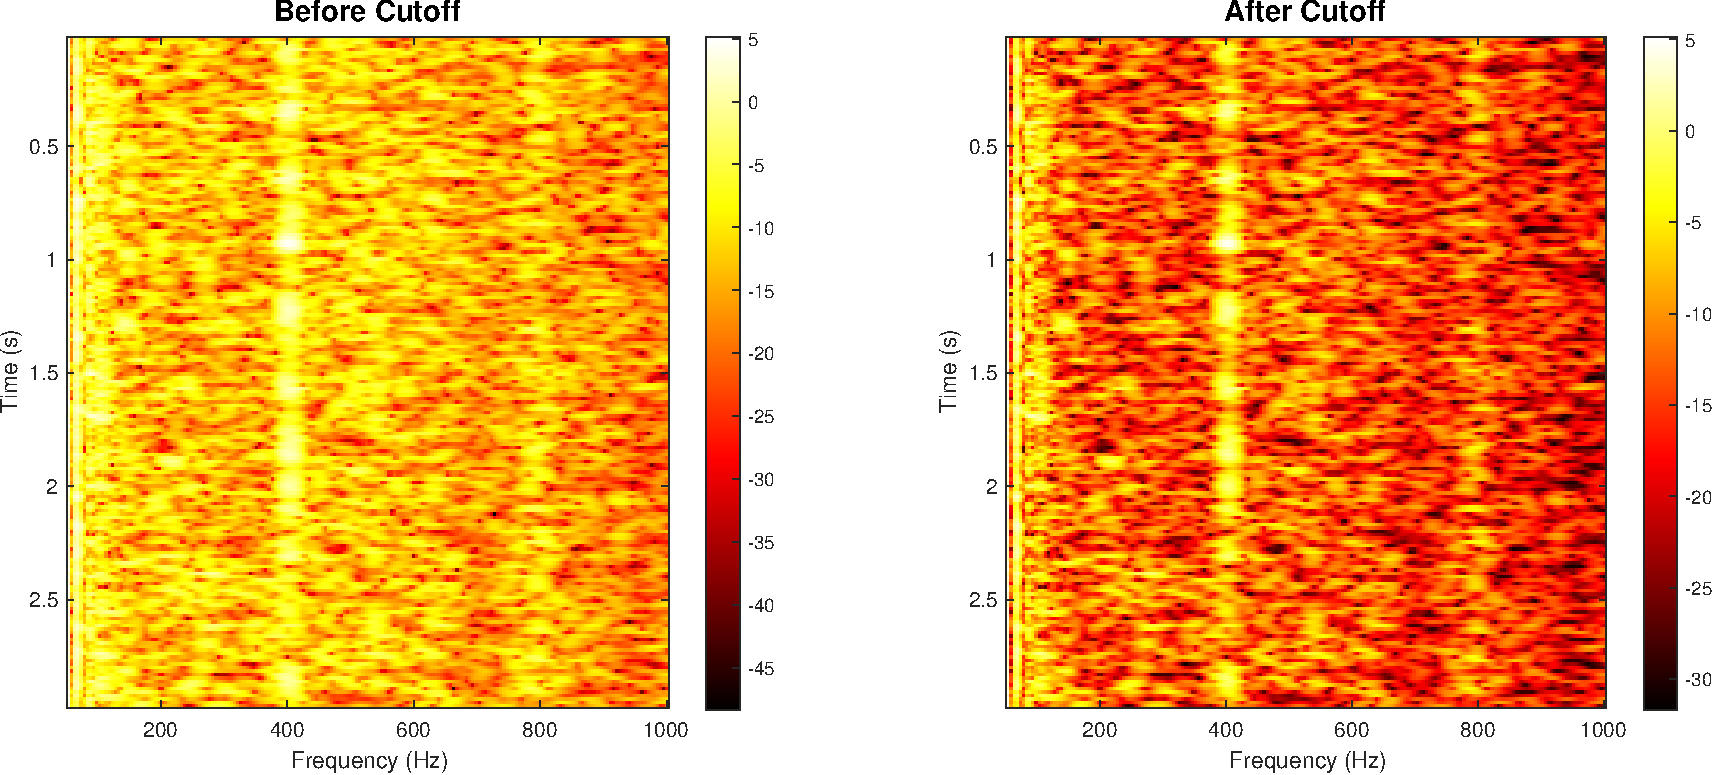
\includegraphics[width=\textwidth]{img/ch3/ampl_cutoff/amplCutoffComparison.pdf}
    \caption{Spectrograms before and after amplitude cutoff. The cutoff at $-30$ dB suppresses low-intensity noise, enhancing visual clarity.}
    \label{fig:ampl-cutoff-spectrogram}
\end{figure}

\subsubsection{Frequency cutoffs}

Two additional preprocessing steps were applied to the power spectrogram matrices to optimise \acrshort{snr} and computational efficiency:

\begin{enumerate}
    \item Low-frequency cutoff: The extremely low-frequency components under 50 Hz were ignored to discard DC offset and other artifacts that do not significantly contribute to vessel classification. By ignoring these components which contain noise and large amplitude variations, the power spectrogram better highlights informative portions of the spectrum, thus improving \acrshort{snr}.
    \item High-frequency cutoff: Based on an analysis of the frequency spectra of each vessel type, a high-frequency cutoff at 1000 Hz was applied. Figure \ref{fig:freq-ampl-highf} shows that for all vessel types analysed (Tug, Cargo, Passengership, and Tanker), significant energy is concentrated below 500 Hz, with a marked decline in amplitude beyond 1000 Hz. By 1500-2000 Hz, the amplitude is nearly negligible, suggesting minimal useful information at these higher frequencies. Setting the cutoff at 1000 Hz allows us to retain the most relevant frequency content while reducing the dimensionality and potential noise in the power spectrogram \cite{premus_machine_2020}. 
\end{enumerate}

\begin{figure}[htbp]
    \centering
    % \begin{subfigure}{0.49\textwidth}
    %     \centering
    %     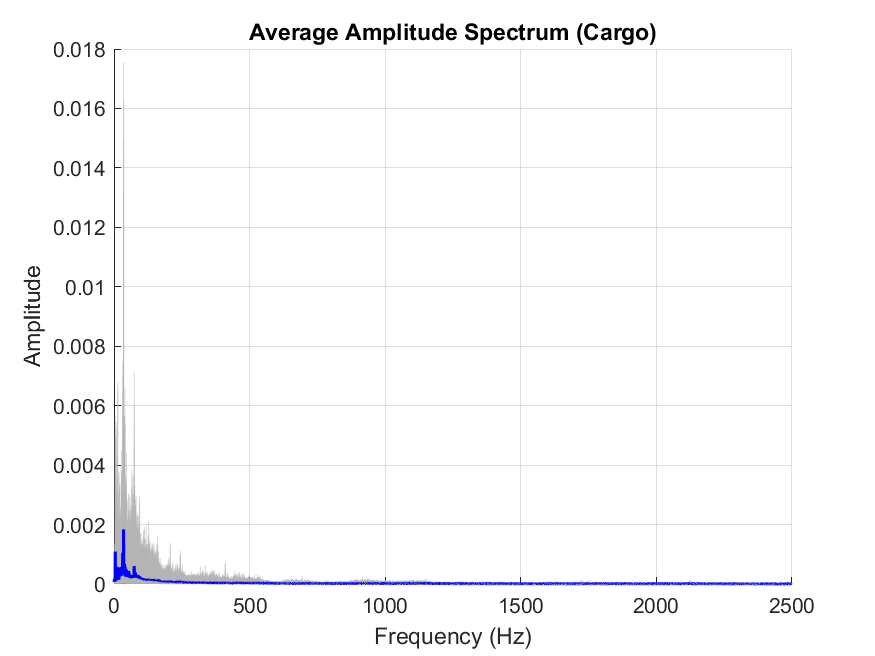
\includegraphics[width=\linewidth]{img/ch3/freq_ampl/cargo_freq_amplitude.png} 
    % \end{subfigure}
    % \hfill
    % \begin{subfigure}{0.49\textwidth}
    %     \centering
    %     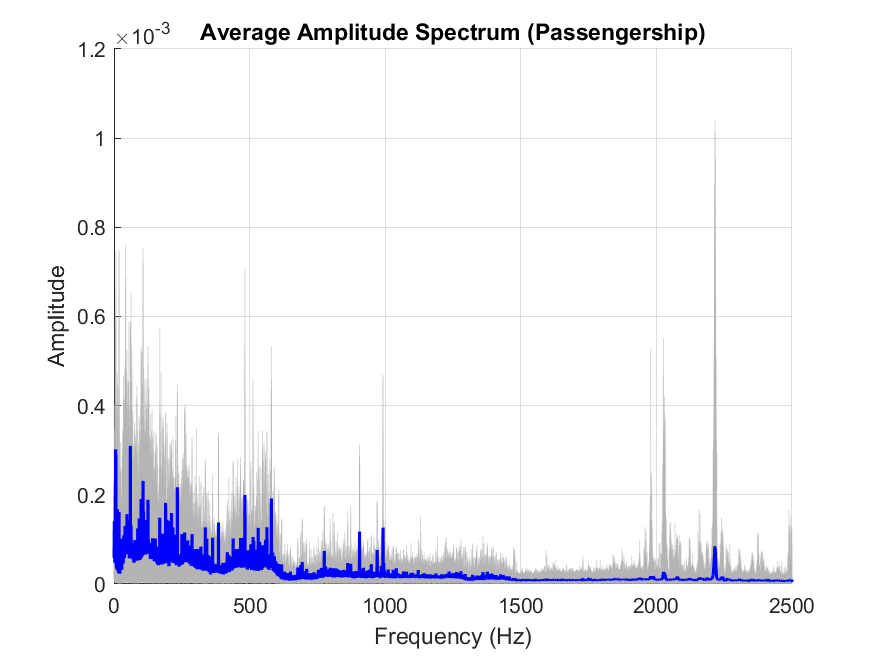
\includegraphics[width=\linewidth]{img/ch3/freq_ampl/passengership_freq_amplitude.png} 
    % \end{subfigure}

    % \vspace{0.5cm} % Space between rows

    % \begin{subfigure}{0.49\textwidth}
    %     \centering
    %     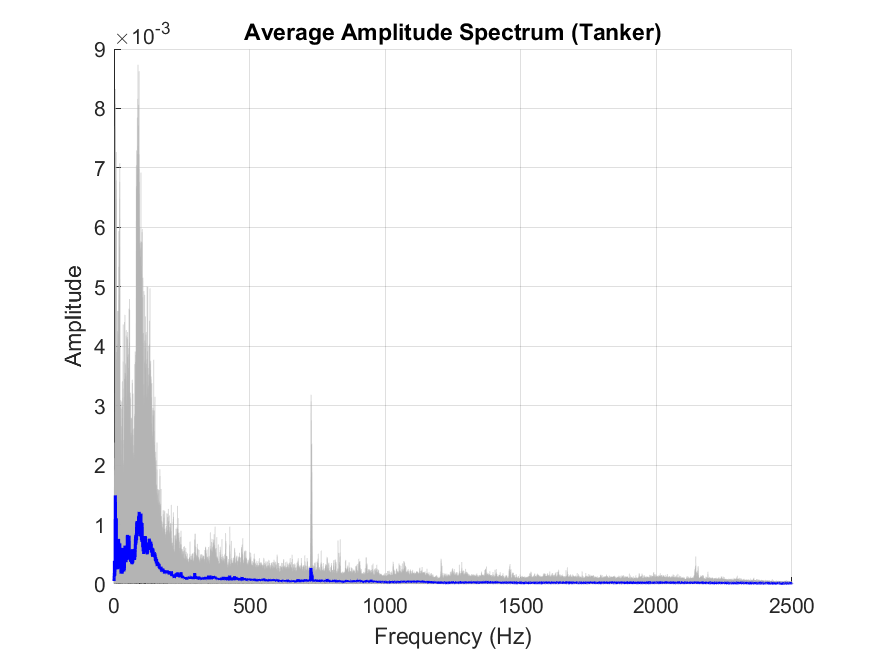
\includegraphics[width=\linewidth]{img/ch3/freq_ampl/tanker_freq_amplitude.png} 
    % \end{subfigure}
    % \hfill
    % \begin{subfigure}{0.49\textwidth}
    %     \centering
    %     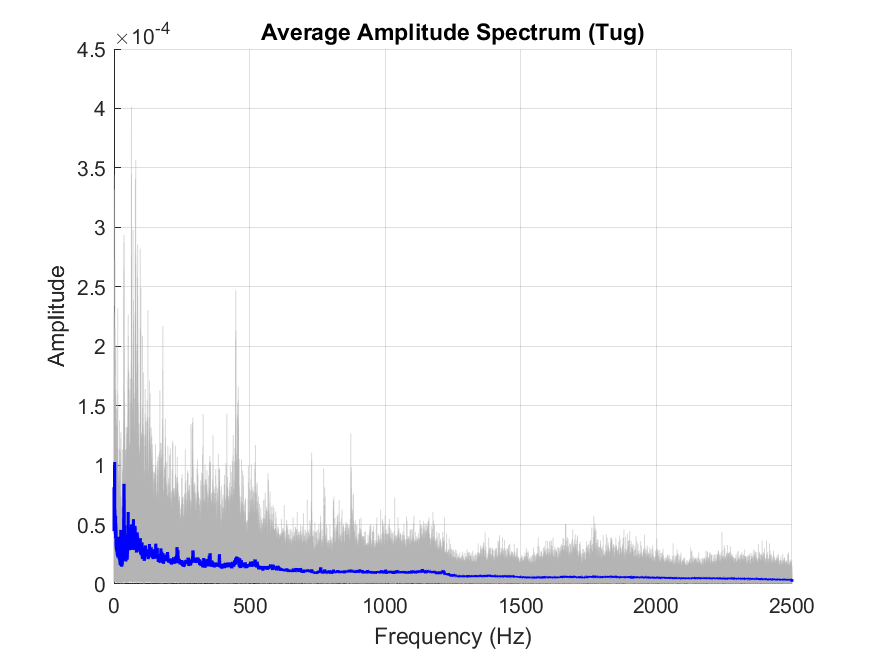
\includegraphics[width=\linewidth]{img/ch3/freq_ampl/tug_freq_amplitude.png} 
    % \end{subfigure}

    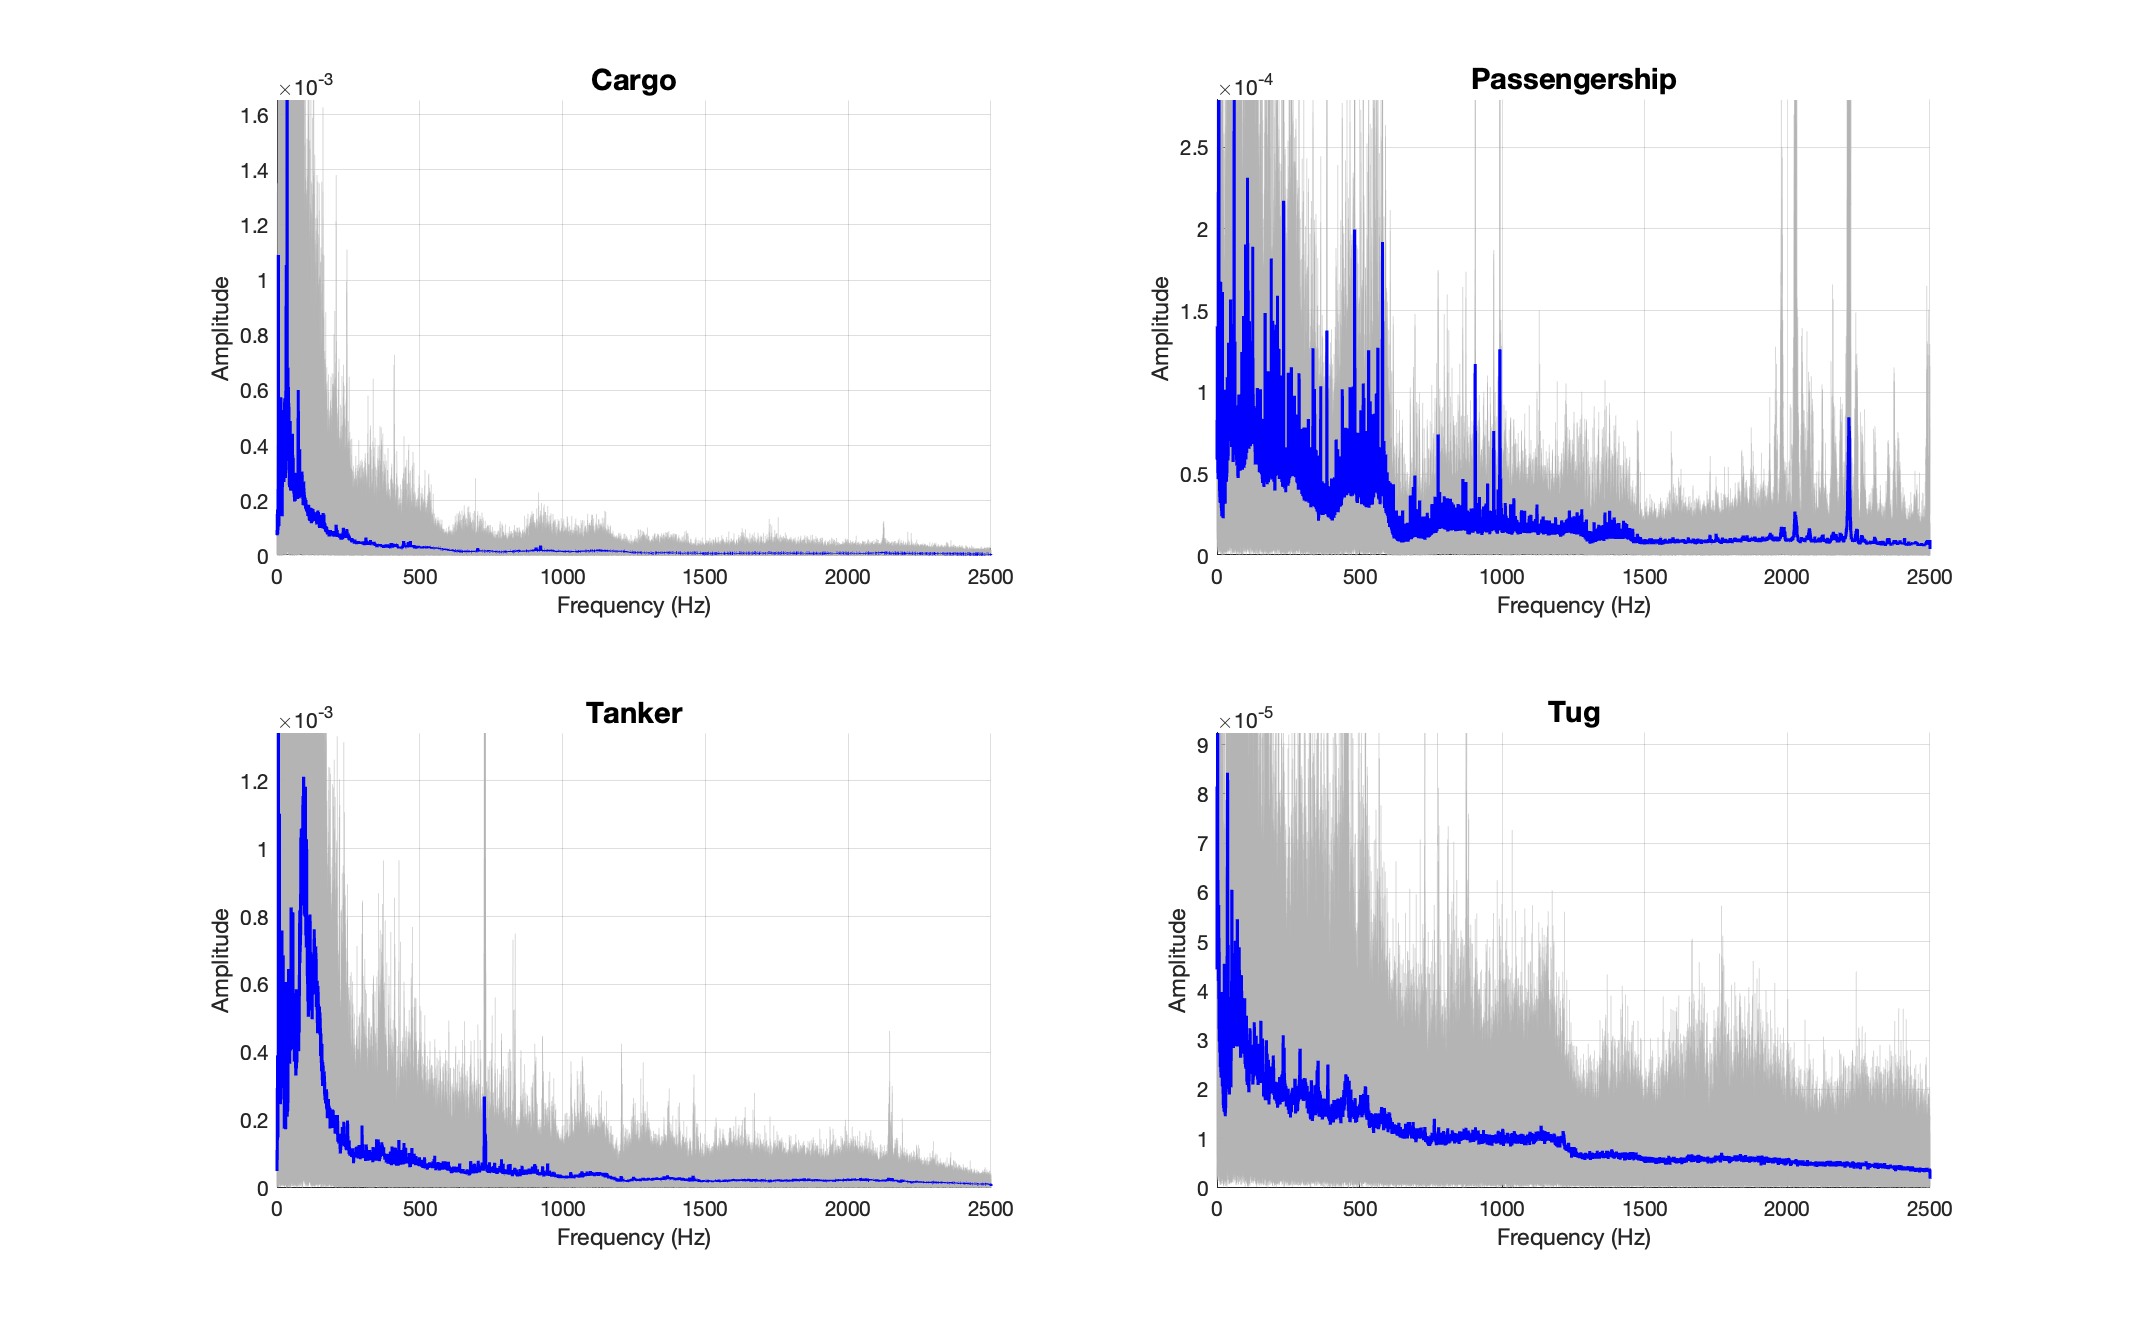
\includegraphics[trim={3.5cm 1cm 2.5cm 1cm},clip,width=\textwidth]{img/ch3/freq_ampl/average_spectra_all.pdf}
    
    \caption{Average single-sided amplitude spectra of each class in the DeepShip dataset. Faint gray lines represent individual segments, while the bold blue line indicates the average amplitude spectrum for each vessel type averaged over 100 segments.}
    \label{fig:freq-ampl-highf}
\end{figure}

\subsubsection{Resizing}

The original spectrogram output had dimensions of $195 \times 231$. In order to ensure compatibility with convolutional layers used in our model, these were resized to $192 \times 192$ using MATLAB's \texttt{imresize} function. The final power spectrogram diagrams which were used as input to the machine learning model are shown in Figure \ref{fig:powerspectrogram-example}.

\begin{figure}[p]
    \centering
    \begin{subfigure}{0.49\textwidth}
        \centering
        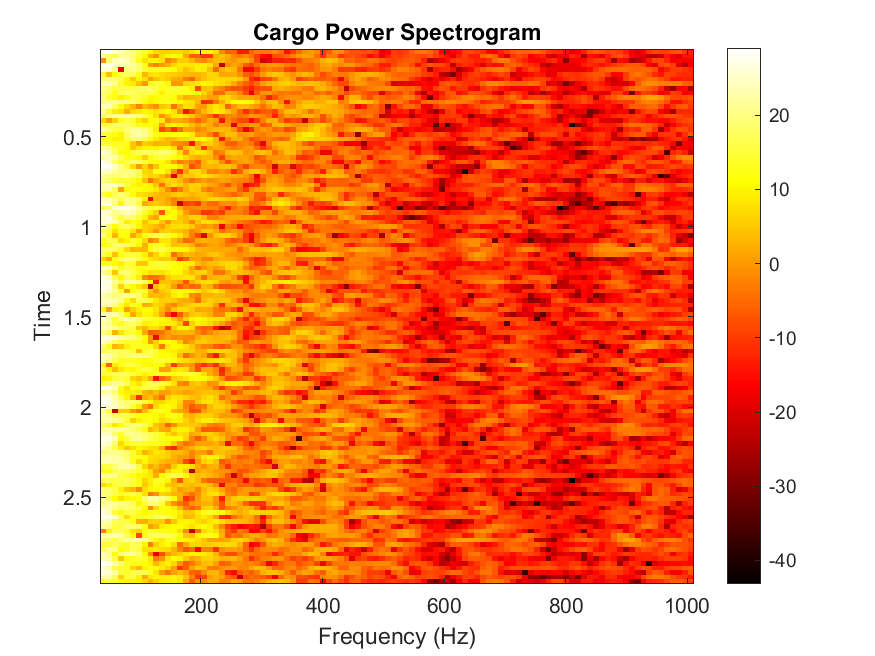
\includegraphics[width=\linewidth]{img/ch3/power_spectrogram/Cargo.png} 
    \end{subfigure}
    \hfill
    \begin{subfigure}{0.49\textwidth}
        \centering
        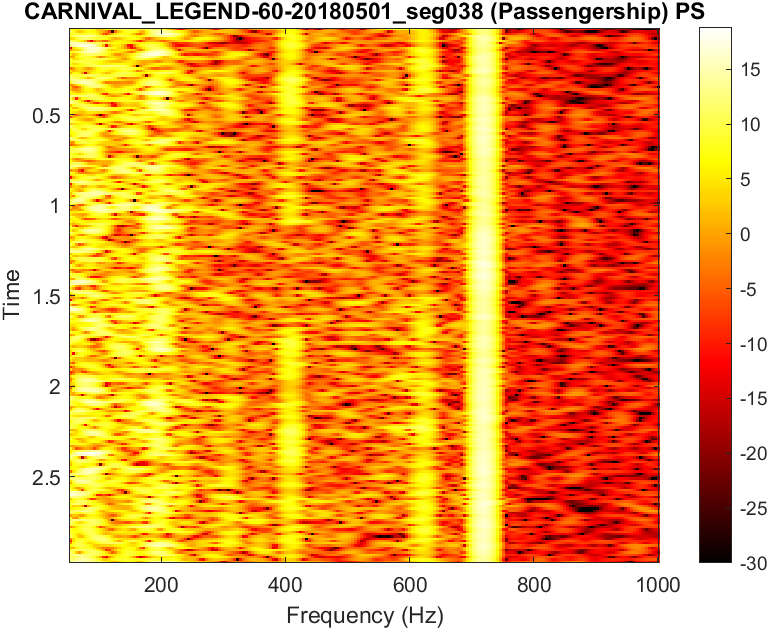
\includegraphics[width=\linewidth]{img/ch3/power_spectrogram/Passengership.png} 
    \end{subfigure}

    \vspace{0.5cm} % Space between rows

    \begin{subfigure}{0.49\textwidth}
        \centering
        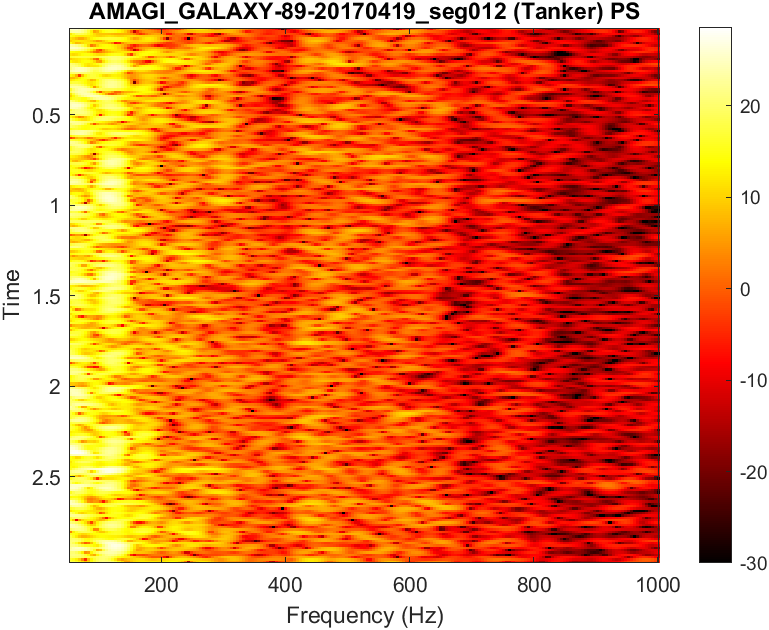
\includegraphics[width=\linewidth]{img/ch3/power_spectrogram/Tanker.png} 
    \end{subfigure}
    \hfill
    \begin{subfigure}{0.49\textwidth}
        \centering
        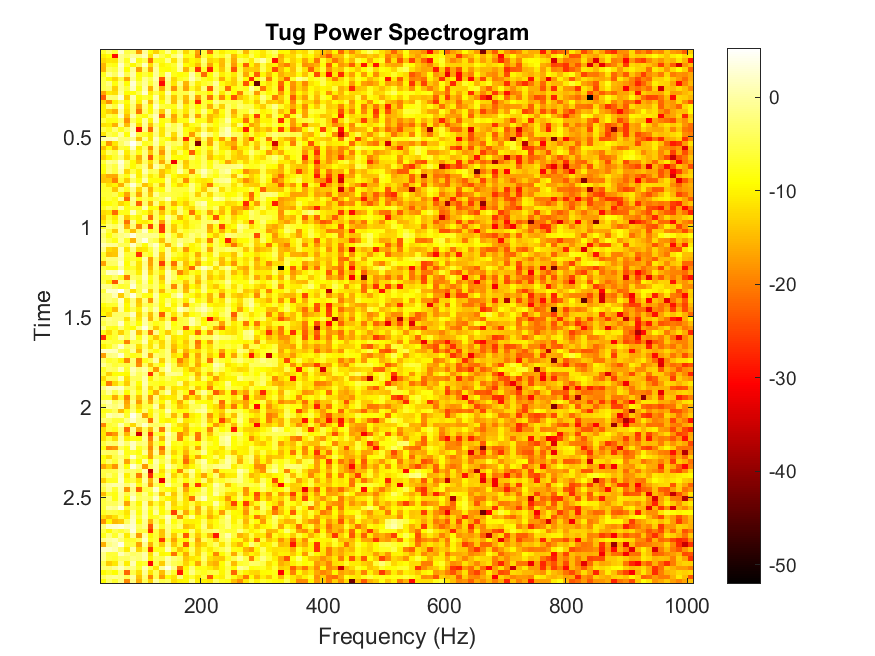
\includegraphics[width=\linewidth]{img/ch3/power_spectrogram/Tug.png} 
    \end{subfigure}
    \caption{Examples of power spectrogram representations for each vessel class in the DeepShip dataset.}
    \label{fig:powerspectrogram-example}
\end{figure}

\subsubsection{Exporting}

To facilitate efficient storage and loading of spectrograms during the model training phase, the computed power spectrograms were exported as \texttt{.mat} files. This choice was made due to the space efficiency of the \texttt{.mat} format compared to CSV files as well as its parsing efficiency with Python via the \texttt{scipy.io.loadmat} function. It achieves this because \texttt{.mat} files store the numerical arrays as structured objects, rather than CSV files which are text-based. This makes it ideal for handling large datasets of spectrogram matrices without excessive file I/O overhead. 

\subsection{Implementation}

The generation of power spectrograms was implemented using MATLAB in a way that ensured flexibility, reproducibility, and clarity in the preprocessing steps. At the core of this pipeline is the custom MATLAB function \texttt{wavToSpec()}, which allows users to specify preprocessing, spectrogram configurations, and export settings through structured parameters. The function accommodates multiple stages of preprocessing, including resampling and frequency cutoffs, with options that can be enabled or adjusted through simple parameter toggles. This modular design not only simplifies experimentation and debugging but also ensures consistency across different stages of the thesis. Additionally, the pipeline serves as an effective documentation tool, enabling future researchers to easily understand and replicate the spectrogram generation process. Its adaptability makes it suitable for processing new datasets or comparing results across varying preprocessing configurations. All related code is available on the project's GitHub page. All MATLAB code was written and tested in version 2024a.

%%%%%%%%%%%%%%%%%%%%%%%%%%%%%%%%%%%%%%%
\section{The classifier: CNN-LSTM}

The chosen classifier for the baseline model is CNN-LSTM, which aims to leverage the strengths of both \acrshort{cnn}s for spatial feature extraction and \acrshort{lstm} networks for sequential data processing. \acrshort{cnn}s excel at analysing spatial data, such as spectrograms of audio signals, while \acrshort{lstm}s are effective at modeling time-series data, identifying temporal patterns across sequences. By integrating CNN and \acrshort{lstm}, the hybrid architecture can capture both spatial and temporal features, making it well-suited for tasks such as time-series forecasting \cite{kim_predicting_2019, lu_cnn-lstm-based_2020}, natural language processing \cite{wang_dimensional_2016, umer_fake_2020}, and (as in our case) image classification in complex domains \cite{vankdothu_brain_2022, islam_combined_2020}. 

In the context of \acrshort{uatr}, this architecture serves as an ideal benchmark due to the spatial and temporal nature of sonar signal data. \acrshort{cnn}s can extract meaningful spatial features from spectrograms, while \acrshort{lstm}s sequentially process these extracted features, capturing unique temporal patterns that vary across vessel types due to differences in machinery, propulsion, and operating speeds. Thus, we believe that the CNN-LSTM classifier is well-positioned to benchmark the DeepShip dataset. 

\subsection{Architecture layout}

\begin{sidewaysfigure}
    \centering
    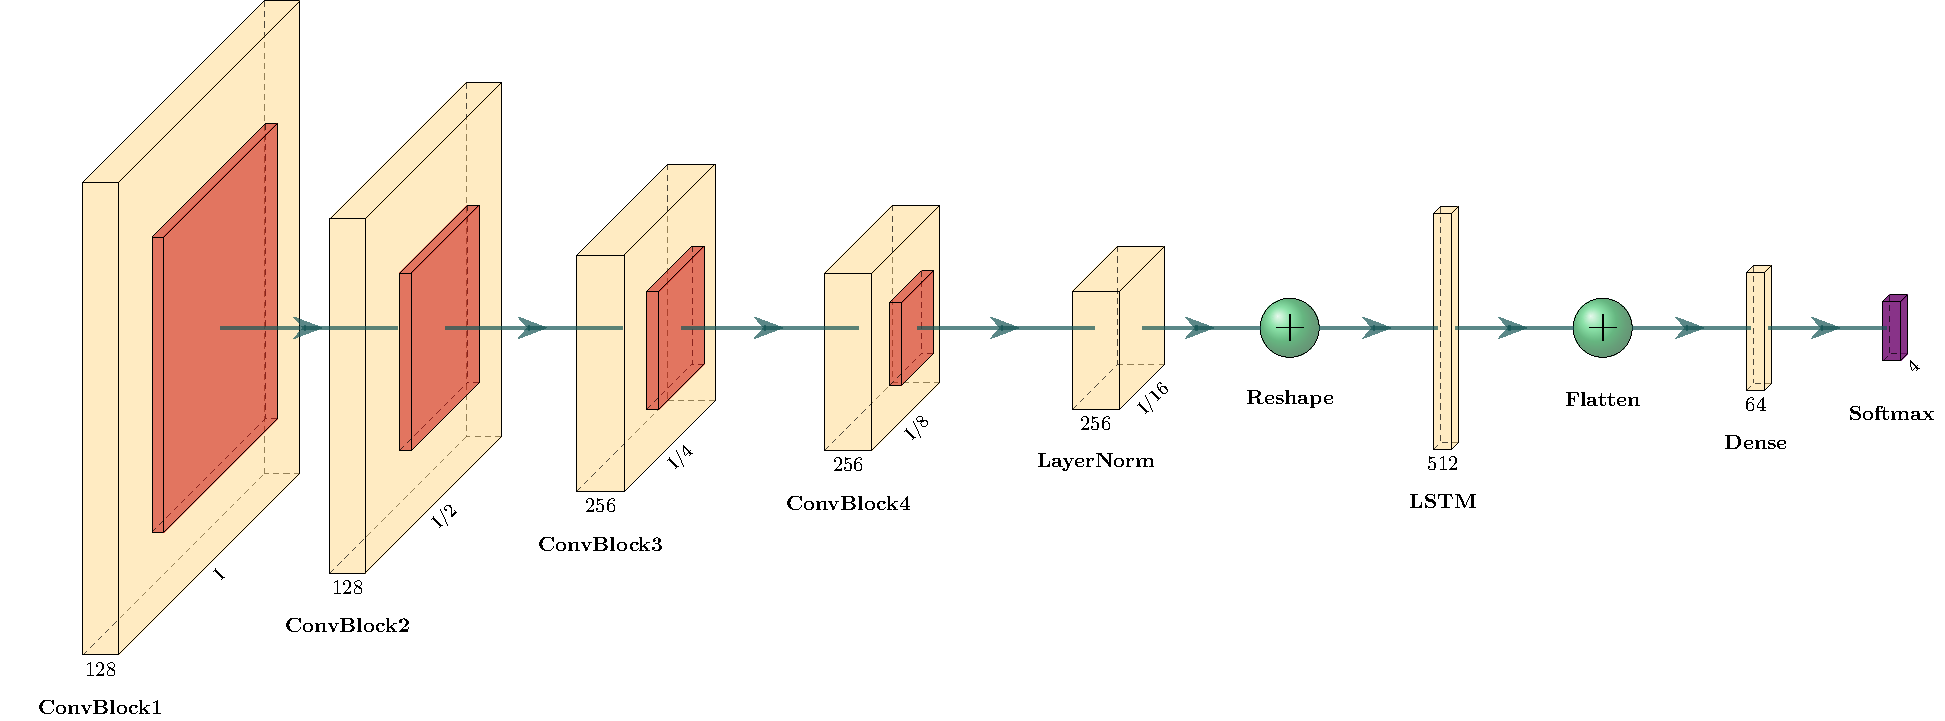
\includegraphics[width=\linewidth]{img/ch3/architecture_diagram.pdf}
    \caption{Baseline CNN-LSTM architecture diagram, illustrating key layers and their configurations. Each ConvBlock includes batch normalisation and ReLU activation, though these are not explicitly shown.}
    \label{fig:cnn-lstm-architecture}
\end{sidewaysfigure}

The architecture starts with four convolutional blocks, each contributing to progressively deeper feature extraction, followed by an \acrshort{lstm} layer for temporal pattern recognition, and concluding with dense layers for final classification. A summary of each component is given below, and a diagram of the network can be found in Figure \ref{fig:cnn-lstm-architecture}.

\paragraph{Convolutional blocks 1 and 2} The first convolutional block applies a 2D convolution layer with 128 filters and a $5\times5$ kernel size, using padding to maintain spatial dimensions. The convolutional layer is followed by batch normalisation, which accelerates training and stabilises the learning process. A ReLU activation function introduces non-linearity, and a $2\times2$ max-pooling layer with a stride of $(2,2)$ down-samples the feature map, reducing spatial dimensions while retaining essential features. The second convolutional block is identical to the first, however, here the max-pooling size is increased to $(4,2)$ to further condense the feature representation.

\paragraph{Convolutional blocks 3 and 4} The third and fourth convolutional blocks replicate the structure of the first two blocks but with double the number of filters to enable the capture of more complex feature hierarchies. Both blocks use a $5\times5$ kernel, batch normalisation, ReLU activation, and max-pooling layers; however, in the final block, the max-pooling layer again uses a larger pooling window $(4, 2)$ to further down-sample the feature map, preparing it for sequential processing.

\paragraph{LSTM layer} After the convolutional blocks, the model incorporates a layer normalisation step to standardise the data. The output is then reshaped before being passed into the \acrshort{lstm} layer with 512 hidden units. The \acrshort{lstm} layer uses the hyperbolic tangent (tanh) as its activation function. This choice is based on TensorFlow's optimisation capabilities; when tanh is used as the activation function, TensorFlow can use an efficient cuDNN implementation on compatible GPUs, accelerating \acrshort{lstm} computations and maximising performance.

\paragraph{Classification layers} Following the \acrshort{lstm} layer, the output is flattened and passed through two fully connected (Dense) layers. The first dense layer, with 64 units and a ReLU activation, reduces the dimensionality and enables more complex learned representations, while the final dense layer, with 4 units and a softmax activation, outputs the class probabilities for the four vessel types under consideration.

\subsection{Training configuration}\label{subsec:training-configuration}

For training, we used a GPU batch size of 16, the Adam optimiser \cite{kingma_adam_2014}, and categorical cross-entropy as the loss function. We set the learning rate to $1 \times 10^{-5}$. 
 
As previously explained, to ensure a robust evaluation of the classifier's performance, we employed a 10-fold leave-two-out cross-validation approach for training. Practically, this meant that each iteration, eight folds were used for training, one fold was used for validation, and one fold was used for testing. This process was repeated 10 times, with each fold serving as the testing set once. The accuracy and loss were averaged across all 10 folds to provide a reliable estimate of the model's performance. This method helps mitigate the potential for overfitting to any specific subset of the data and provides a more comprehensive measure of the classifier's generalisation ability. A summary of the final training parameters can be found in Table \ref{tab:cnn-lstm-final-params}. 

All training was conducted on a Windows machine equipped with a NVIDIA GeForce RTX 2080 GPU (8GB) and 64GB of RAM, which provided sufficient computational resources for handling the dataset and training iterations. The baseline model was implemented using TensorFlow Keras (v2.10.0), and trained with CUDA (version 12.6), cuDNN (version 8.1.0), and cudatoolkit (version 11.2) libraries which are necessary for accelerated deep learning on NVIDIA GPUs. 

\begin{table}[htb]
\centering
\begin{tabular}{ll}
\toprule
\textbf{Parameter} & \textbf{Final value} \\ \midrule
GPU batch size & 16 \\
Optimiser & Adam \\
Loss function & Categorical cross-entropy \\
Learning rate & $1 \times 10^{-5}$ \\
Validation approach & Leave-two-out 10-fold cross validation \\
Evaluation metrics & Accuracy, F1-score \\ \bottomrule
\end{tabular}
\caption{Final training parameters for benchmark CNN-LSTM model.}
\label{tab:cnn-lstm-final-params}
\end{table}

\subsection{Hyperparameter tuning}

The final architecture and training configuration described in the preceding sections were determined through an iterative process of hyperparameter tuning. Initially, the model architecture was designed with parameters based on standard practices for \acrshort{cnn}s and \acrshort{lstm} layers for time-series and spectral data. Specifically, the CNN layers used a filter size of $3 \times 3$ with 64 filters, while the \acrshort{lstm} layer included 1024 hidden units. The learning rate for training was set at $1 \times 10^{-3}$. However, we employed the Keras Tuner library to try and enhance our architecture and configuration. 

We used Keras Tuner's \texttt{RandomSearch} method for hyperparameter tuning. Random search is particularly well-suited for projects with large search spaces and limited computation resources, as alternative methods (such as Bayesian optimisation) often require the direct modelling of dependencies between parameters -- a computationally expensive step. Using random search allowed us to find the most promising configurations in a relatively short time.

The hyperparameters included in the search space, as well as a brief motivation for tuning each of them, is provided below. 

\begin{itemize} 
\item Number of filters and filter size: We tested kernel sizes of length $[3, 5, 7]$ to evaluate how receptive field size affects the model's ability to capture spatial features. We also varied the number of filters in each convolutional layer across $[32, 64, 128, 256]$.
\item LSTM units: We tested \acrshort{lstm} configurations with 
$[256, 512, 1024, 2048]$ units to determine the optimal memory capacity for capturing temporal dependencies. 
\item Dense layer units and activation function: For the dense layer immediately after \acrshort{lstm}, we experimented with $[32, 64, 128, 256]$ units and evaluated both \texttt{relu} and \texttt{tanh} activations to observe which non-linearity best captures high-level abstractions in the data. 
\item Optimiser: The choice of optimiser can significantly impact convergence; we compared \texttt{adam}, \texttt{rmsprop}, and \texttt{sgd}. 
\item Learning rate: Four different learning rates were tested to find the best balance between learning speed and stability: $1 \times 10^{-5}$, $1 \times 10^{-4}$, $1 \times 10^{-3}$ and $1 \times 10^{-2}$.
\end{itemize}

A summary of the search space alongside the hyperparameter configuration yielding the best performance is provided in Table \ref{tab:hyperparameter-search-space}.

\begin{table}[htbp] 
\centering 
    \begin{tabular}{lll} 
    \toprule 
    \textbf{Hyperparameter} & \textbf{Values tested} & \textbf{Optimal value} \\ 
    \midrule 
    Filter size (\texttt{filter\_size}) & 3, 5, 7 & 5 \\ 
    Number of filters (\texttt{num\_filters}) & 32, 64, 128, 256 & 128 \\ 
    LSTM units (\texttt{lstm\_units}) & 256, 512, 1024, 2048 & 512 \\ 
    Dense layer units (\texttt{dense\_units}) & 32, 64, 128, 256 & 64 \\ 
    Dense layer activation (\texttt{dense\_activation}) & \texttt{relu}, \texttt{tanh} & \texttt{relu} \\ 
    Optimiser (\texttt{optimizer}) & \texttt{adam}, \texttt{rmsprop}, \texttt{sgd} & \texttt{adam} \\ 
    Learning rate (\texttt{learning\_rate}) & 1e-5, 1e-4, 1e-3, 1e-2 & $1 \times 10^{-5}$ \\ 
    \bottomrule 
    \end{tabular} 
\caption{Hyperparameter search space used for model tuning with ideal configuration.} 
\label{tab:hyperparameter-search-space} 
\end{table}

These results highlight that a larger filter size and an increased number of filters in the \acrshort{cnn} layers improved the model's feature extraction capability, while a reduction in \acrshort{lstm} units (from the initial 1024 to 512) helped balance memory capacity with computational efficiency. Additionally, a low learning rate of $1 \times 10^{-5}$ with the Adam optimiser yielded the best results.

Based on these results, the final network architecture was modified to incorporate the optimal hyperparameters. The \acrshort{cnn} was configured with a $5\times5$ filter size and 128 filters, while the \acrshort{lstm} layer used 512 hidden units. The dense layer was set to 64 units with \texttt{relu} activation. Training was carried out with the Adam optimiser and a learning rate of $1 \times 10^{-5}$. This process of hyperparameter tuning not only improved the model's performance but also provided insights into the configuration choices that best capture the temporal and spectral features for \acrlong{uatr}.

\section{Implementation}

The implementation of the CNN-LSTM classifier and training pipeline was built around a reusable and flexible TensorFlow Keras-based codebase. Key features of this implementation are its adaptability to large datasets as well as its ability to perform $k$-fold cross-validation. 

\subsection{Dataset handling}

Given the dataset's size of over 53,000 segments, making up over 25GB of data, a critical bottleneck in the DeepShip machine learning pipeline was the handling of spectrogram data. The primary challenge lay in the process of loading spectrogram data from files into memory, which is computationally expensive and prone to causing memory issues if not optimised. This led to a progressive evolution of strategies to optimise data loading in order to ensure stability during training. Over the course of this thesis, three distinct approaches were explored, each improving on its predecessor in terms of efficiency and practicality.

The first approach was the most naive: the entire dataset was loaded into memory as NumPy arrays at the start of the script. While this method was simple to implement, it quickly became apparent that it was impractical for datasets of this scale. Both RAM and GPU memory usage would exceed the capacity of the machine we were training on, leading to frequent \texttt{ResourceExhaustedError}'s during training. While this approach allowed initial experimentation with the machine learning pipeline, its limitations called for a more sophisticated solution.

The second attempt involved using TensorFlow's \texttt{tf.Dataset} API, which introduced some level of optimisation by delaying the loading of data into memory until the start of each fold. Specifically, the dataset corresponding to fold 1 would only be loaded at the beginning of fold 1, and the process would repeat for subsequent folds. While this approach reduced the memory footprint compared to the naive method, it still required loading an entire fold's dataset at once, which often exceeded memory limits. Moreover, training curves and performance metrics exhibited odd inconsistencies, which led to us abandoning the method.

The third and final approach involved implementing custom data generators, which dynamically load and preprocess spectrogram data in small batches just before it is fed into the model. This strategy introduced a parameter, \texttt{DATA\_BATCH\_SIZE}, controlling how many spectrograms are read from disk and converted into NumPy arrays at any given time. Unlike previous strategies, this approach delayed the spectrogram parsing step until the very last moment, significantly reducing memory usage and enabling stable, uninterrupted training. By only loading \texttt{DATA\_BATCH\_SIZE} spectrograms into memory at a time, the custom generators not only avoided memory bottlenecks but also provided flexibility to scale the pipeline for larger datasets or limited hardware configurations. Ultimately, these custom data generators became the foundation of our DeepShip machine learning pipeline, ensuring efficient and reliable data handling while still maximising resource utilisation. 

\subsection{\texorpdfstring{$k$}{k}-fold Cross-Validation}

The central component of the training pipeline is the \texttt{k\_fold\_cross\_validation} function, handling the partitioning of the dataset and the iterative training, validation, and testing process. For each fold, the dataset is divided such that the current fold serves as the test set, the next fold (or the first fold, if at the last iteration) is used for validation, and the remaining folds are used for training. This ensures that each fold is utilised for testing exactly once, providing a comprehensive evaluation of the model's performance.

The aforementioned data generators then dynamically load and preprocess the spectrograms in batches just before they are fed into the model, avoiding memory overload and allowing control over parameters like batch size and shuffling. The model's performance is evaluated using metrics such as loss, accuracy, precision, recall, and F1-score. These metrics are calculated for each fold and averaged to summarise the model's overall performance. The model weights are reset each fold, ensuring a robust and thorough assessment of the model and a reliable method for benchmarking performance.

\section{Benchmark results}

\subsection{Initial experiment: 5 epochs}

After training the benchmark CNN-LSTM model with the final parameters detailed in Table~\ref{tab:cnn-lstm-final-params} for 5 epochs per fold, we achieved an \textbf{overall baseline accuracy of 89.07\%}. The model also demonstrated strong performance across key classification metrics, with an average precision of 90.22\%, recall of 89.07\%, and F1 score of 89.16\%.

The training and validation accuracy and loss curves, shown in Figure~\ref{fig:baseline5-acc-loss}, provide insight into the model's performance across the 10-fold cross-validation process. Notably, the validation loss began to increase after the third epoch, accompanied by a corresponding decrease in validation accuracy. This pattern strongly suggests that the model was overfitting to the training data after the third epoch. Hence, while the metrics achieved with this configuration were highly encouraging, the observed signs of overfitting prompted further investigation.

\begin{figure}[p]
    \centering
    
    % Subfigure 1: Validation metrics by epoch
    \begin{subfigure}[t]{\textwidth}
        \centering
        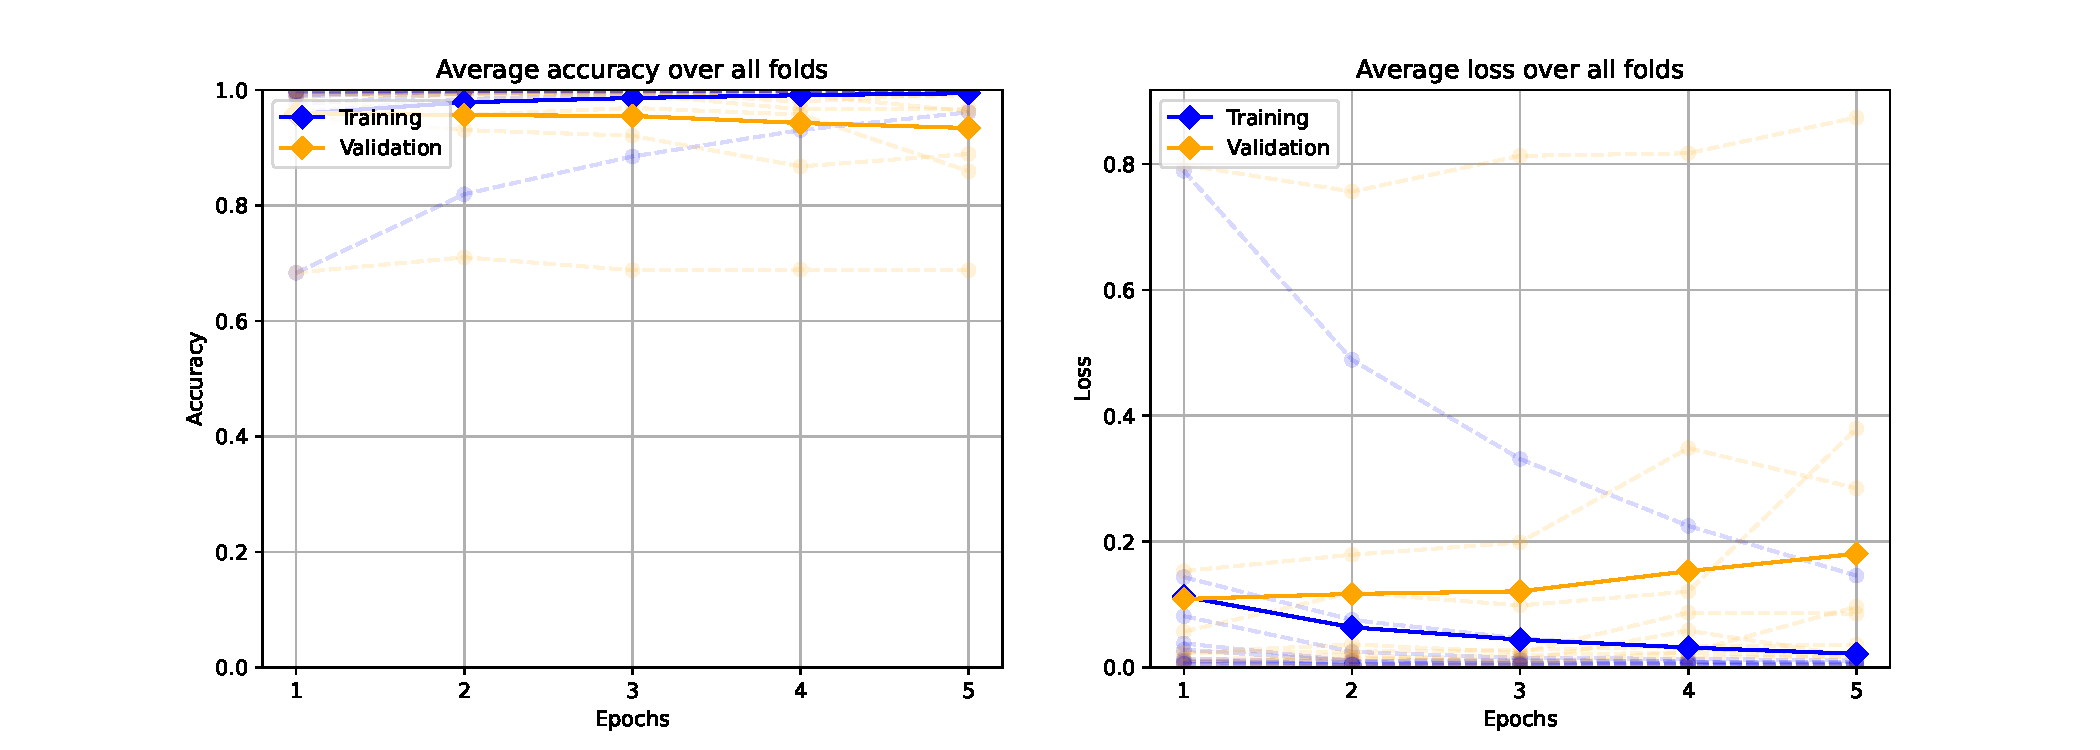
\includegraphics[trim={3cm 0 3cm 0.8cm},clip,width=\textwidth]{img/ch3/baseline_results/5_epochs_by_epoch.pdf}
        \caption{Validation accuracy and loss across all folds by epoch.}
        \label{fig:baseline5-by-epoch}
    \end{subfigure}
    
    \vspace{0.5cm}
    
    % Subfigure 2: Validation metrics by fold
    \begin{subfigure}[t]{\textwidth}
        \centering
        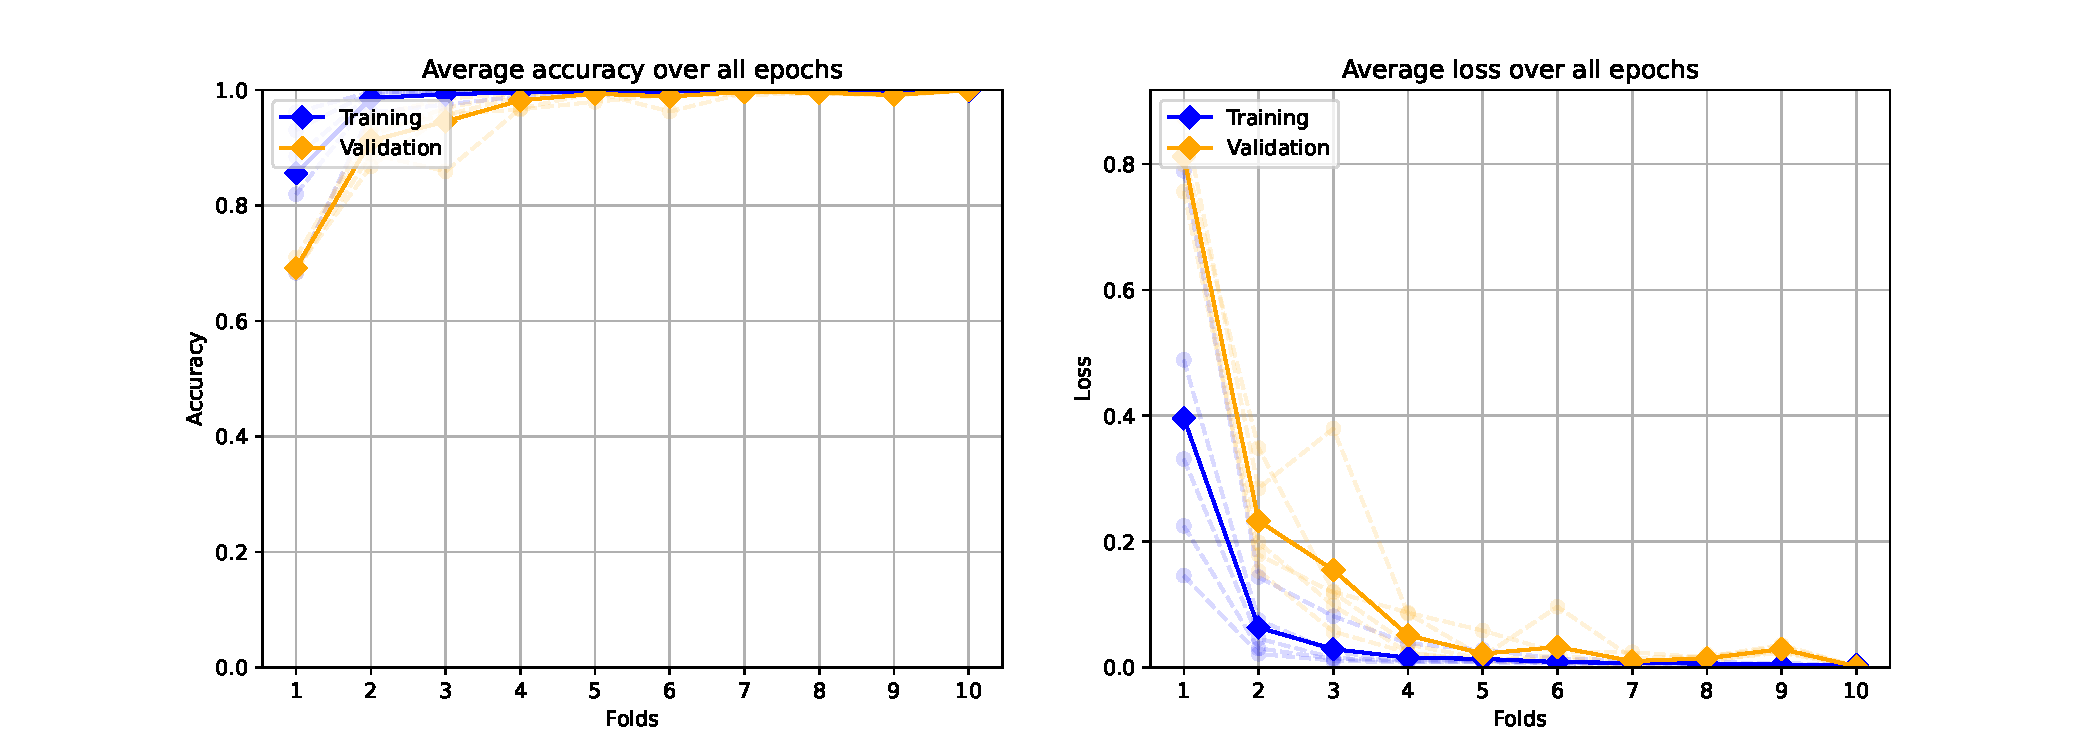
\includegraphics[trim={3cm 0 3cm 0.8cm},clip,width=\textwidth]{img/ch3/baseline_results/5_epochs_by_fold.pdf}
        \caption{Validation accuracy and loss across all epochs by fold.}
        \label{fig:baseline5-by-fold}
    \end{subfigure}
    
    \caption{Training and validation accuracy and loss for the benchmark CNN-LSTM model during the initial experiment with 5 epochs.}
    \label{fig:baseline5-acc-loss}
\end{figure}

\subsection{Final benchmark: 3 epochs}

\begin{figure}[p]
    \centering
    
    % Subfigure 1: Validation metrics by epoch (3 epochs)
    \begin{subfigure}[t]{\textwidth}
        \centering
        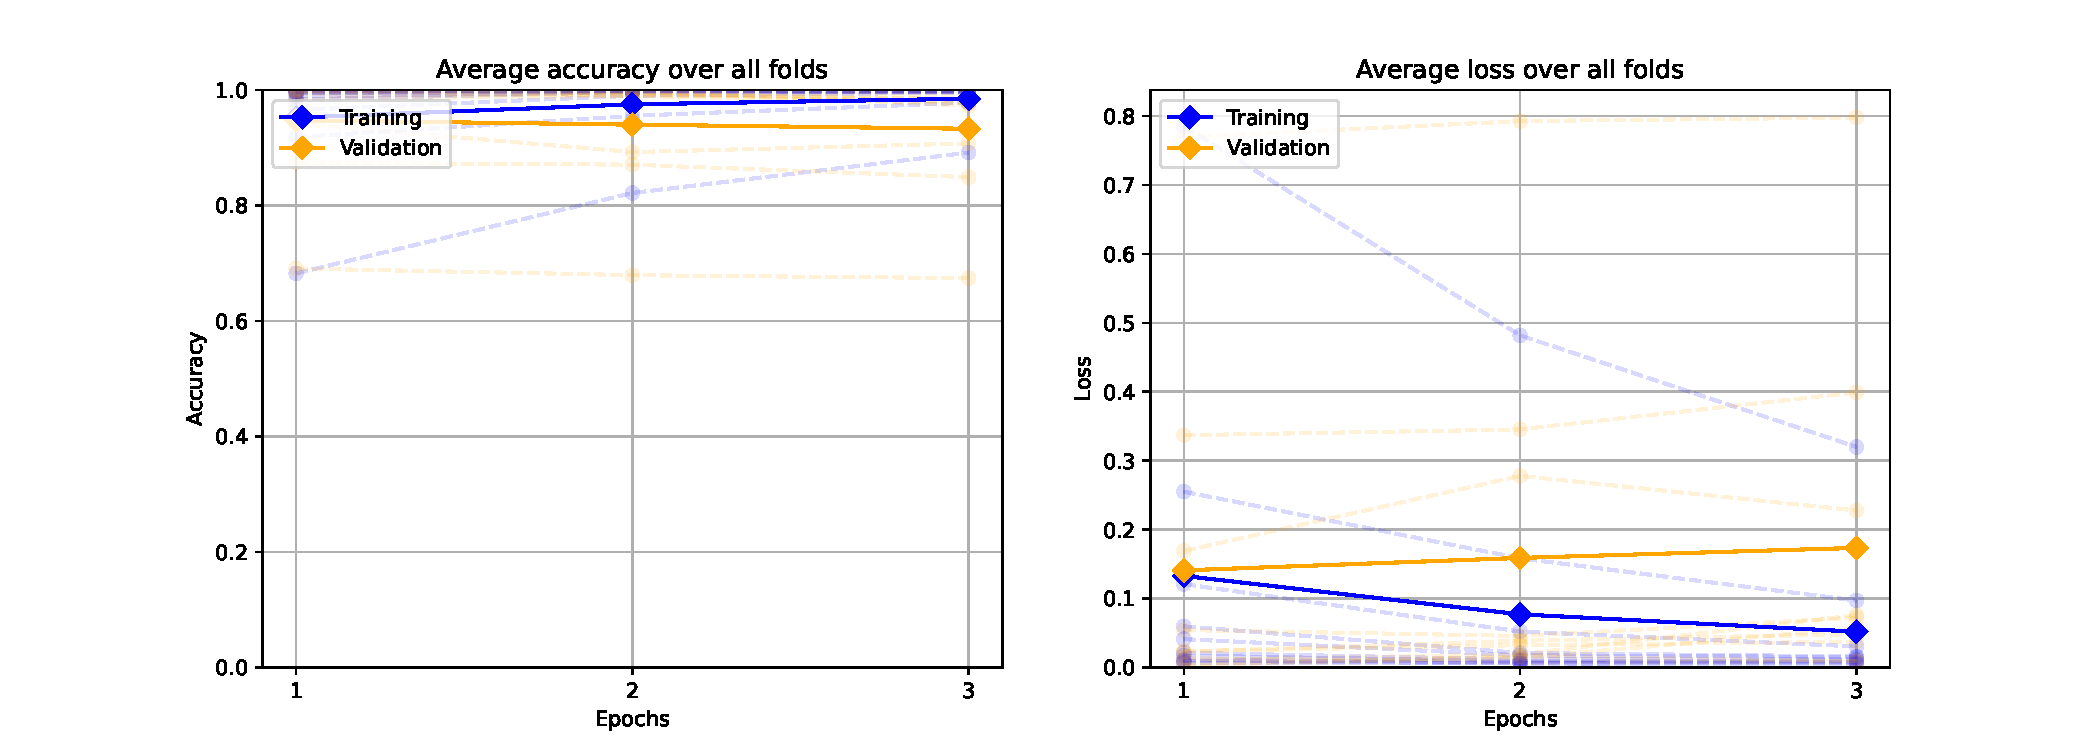
\includegraphics[trim={3cm 0 3cm 0.8cm},clip,width=\textwidth]{img/ch3/baseline_results/3_epochs_by_epoch.pdf}
        \caption{Validation accuracy and loss across all folds by epoch.}
        \label{fig:baseline3-by-epoch}
    \end{subfigure}
    
    \vspace{0.5cm}
    
    % Subfigure 2: Validation metrics by fold (3 epochs)
    \begin{subfigure}[t]{\textwidth}
        \centering
        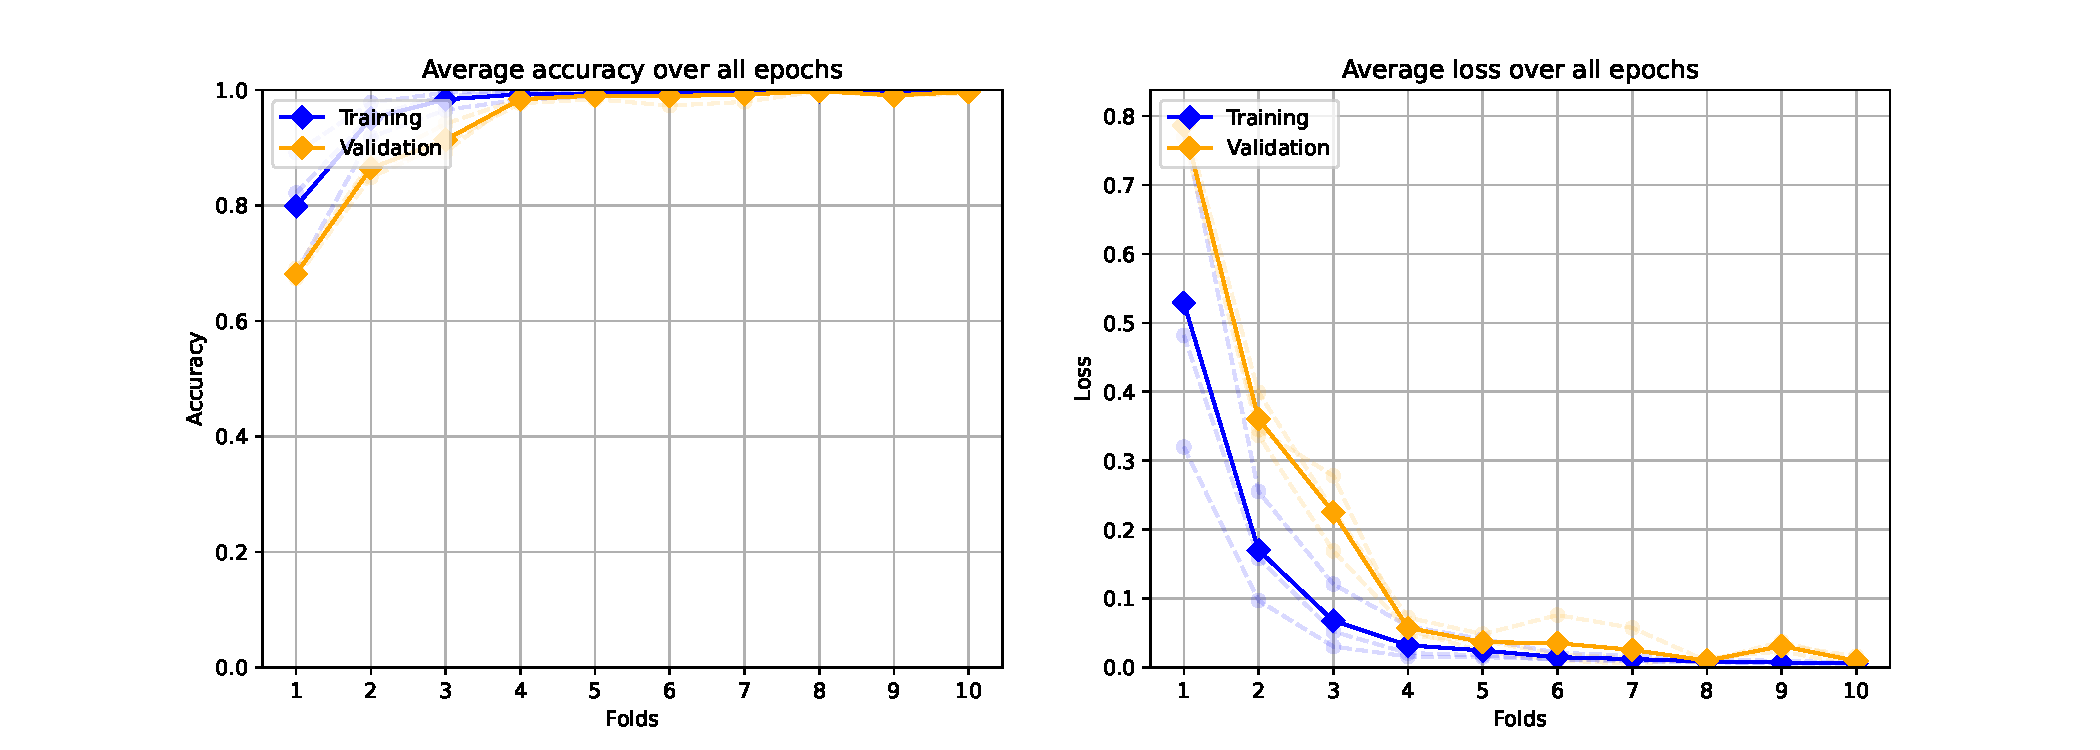
\includegraphics[trim={3cm 0 3cm 0.8cm},clip,width=\textwidth]{img/ch3/baseline_results/3_epochs_by_fold.pdf}
        \caption{Validation accuracy and loss across all epochs by fold.}
        \label{fig:baseline3-by-fold}
    \end{subfigure}
    
    \caption{Training and validation accuracy and loss for the benchmark CNN-LSTM model retrained with 3 epochs.}
    \label{fig:baseline3-acc-loss}
\end{figure}

To address the overfitting observed in the initial experiment, we retrained the CNN-LSTM model using the same 10-fold cross-validation setup but reduced the training duration to 3 epochs per fold. This adjustment aimed to limit overfitting and improve the model's generalisation performance.

After retraining, the model achieved an \textbf{overall baseline accuracy of 87.94\%}, with an average precision of 88.78\%, recall of 87.94\%, and F1 score of 88.03\%. While there was a slight decrease in accuracy compared to the initial 5-epoch experiment, the validation loss and accuracy curves were much more stable across epochs, as shown in Figure~\ref{fig:baseline3-acc-loss}. Notably, the validation accuracy no longer exhibited the pronounced decline seen in the earlier experiment, and the validation loss remains generally constant throughout training, indicating that the shortened training duration helped mitigate the overfitting effect to a certain extent.

In conclusion, while the average accuracy decreased slightly compared to the inital 5-epoch experiment, the final accuracy of \textbf{87.94\%} provides a more robust and reliable baseline for future experimentation with preprocessing techniques and feature inputs. These results highlight the importance of monitoring validation metrics in an attempt to strike a balance between performance and generalisation.

